\chapter{Implementación del núcleo de la aplicación móvil}\label{cap:implementacion}
Para la implementación del prototipo básico del núcleo básico de la aplicación móvil del sistema ALERTAR se utilizó TypeScript como lenguaje de programación y React Native como librería para el desarrollo de la aplicación sobre sistemas operativos móviles Android e iOS. Además, como sistema gestor de bases de datos se utilizó SQLite. Se utilizó una arquitectura limpia para asegurar la mantenibilidad y escalabilidad del código. Esto permitió la separación de aspectos y la implementación de principios SOLID \cite{martin2003agile}, mejorando la calidad del software.

Los desafíos de la implementación del prototipo de núcleo del sistema ALERTAR se detallan en la sección \ref{sec:desafiosImpl}. La implementación de un mecanismo de autenticación de dispositivos y cómo se garantiza la seguridad de las comunicaciones se explica en la sección \ref{sec:autentic_seguridad}. Una breve descripción del propósito de cada mensaje del protocolo de comunicación de nivel de aplicación utilizado está detallado en la sección \ref{sec:protocoloComunicacion}. La implementación de un gestor de mensajes discretos de nivel de aplicación es desarrollada en la sección \ref{sec:packageManager}. En la sección \ref{sec:perdidaConect}, se explica la definición y puesta en marcha de un mecanismo de detección de pérdida de conectividad de dispositivos. En la sección \ref{sec:serializacion} se detalla cómo es que se evitan errores de concurrencia al ejecutar operaciones relacionadas a los casos de uso. Por último, en la sección \ref{sec:implementacion} se describe la arquitectura propuesta de la aplicación, y se especifica la implementación realizada de casos de uso representativos.

\section{Desafíos de la implementación}

\label{sec:desafiosImpl}
Dada la naturaleza de la aplicación, donde se requiere que los mensajes lleguen en orden y sin errores, se elige TCP como protocolo de transporte. Además, ante la dificultad que presentan las redes de comunicaciones para establecer conexiones en el sentido del servidor hacia clientes, se decidió usar conexiones persistentes a fin de mantener canales de comunicación abiertos entre componentes del sistema.

Se requiere del establecimiento de un canal seguro de comunicación que contemple la confidencialidad, integridad y autenticidad de los datos. A causa de esto, se adoptó el protocolo TLS \textit{(Transport Layer Security)}.

La aplicación trabaja con mensajes discretos, pero al utilizar TCP se tiene un flujo de bytes. Por ello, es necesario un mecanismo que permita al receptor identificar en qué byte comienza y termina un mensaje. Inicialmente se consideró el uso de WebSocket \cite{fette2011websocket} ya que garantiza una conexión persistente, bidireccional y de baja latencia, sumado que los datos se transmiten como mensajes discretos. Además, opera sobre el protocolo TCP y hace uso de TLS para proveer seguridad de las comunicaciones. Sin embargo, se encontró una limitación en el contexto de React Native: la falta de librerías adecuadas. React Native no implementa WebSocket de manera nativa, por lo que hace uso de librerías de terceros. ALERTAR requiere que los dispositivos móviles de la capa de niebla actúen como servidores, pero ninguna de las librerías de WebSocket ofrece soporte para esta configuración. Todas las implementaciones existentes presuponen la presencia de servidores convencionales ejecutándose en computadoras dedicadas, excluyendo a dispositivos móviles.

Descartado el uso de WebSocket se optó por implementar un protocolo de discretización de mensajes sobre TLS/TCP, utilizando la librería $react\_native\_tcp\_socket$ \cite{react-native-tcp-socket}.

TLS utiliza certificados digitales para distribuir claves públicas y autenticar a las partes. En el caso de ALERTAR, los roles de cliente y servidor pueden cambiar dinámicamente, lo que impide depender de servidores fijos con certificados preestablecidos. Por esta razón, fue necesario diseñar e implementar un esquema dinámico para la distribución y validación de certificados, que permita asegurar las comunicaciones en un entorno donde los dispositivos pueden asumir distintos roles de forma flexible.

Por último, si bien el protocolo TCP define mecanismos para la detección de fallos de conexión, la librería $react\_native\_tcp\_socket$ presenta problemas para informar de manera apropiada e inmediata los fallos. Específicamente, cuando un dispositivo móvil pierde su conexión Wi-Fi o de datos móviles, la biblioteca no logra detectar la desconexión. A causa de esto, fue necesaria la implementación de un mecanismo de detección de pérdida de conectividad.

\section{Mecanismo de autenticación de dispositivos y seguridad de las comunicaciones}
\label{sec:autentic_seguridad}
En el sistema ALERTAR, los certificados son emitidos por dos entidades diferentes por un lado, una entidad certificante externa que genera y firma el certificado de la nube, y por otro lado, la nube es la encargada de la generación y firma de los certificados de los dispositivos móviles.

El proceso de manera resumida es el que se enumera a continuación y es el mismo planteado en la Figura \ref{fig:CADist}. Además es importante tener en cuenta el proceso de \textit{handshake TLS} explicado en la figura \ref{fig:handshakeTLS}.
\begin{enumerate}
    \item El dispositivo de borde envía un mensaje \textit{``hello''} a la nube.
    \item La nube responde con su certificado.
    \item El dispositivo de borde verifica que ese certificado esté firmado por alguna entidad certificante de confianza.
    \item Si el certificado es válido continúa el proceso de \textit{handshake TLS}.
\end{enumerate}

Cada dispositivo móvil tiene un único certificado. Este es otorgado por la nube en el momento en que el primer usuario que utiliza la aplicación hace un inicio de sesión. Por lo tanto, la primera vez que se realiza un inicio de sesión en cada dispositivo, es necesario que posea conexión a Internet para poder recibir su certificado desde la nube. Este certificado se entrega a través de un canal seguro entre el dispositivo de borde y la nube, lo cual evita un ataque tipo ``Hombre en el medio''. Esto se puede realizar de las siguientes dos maneras:

\begin{itemize}
    \item \textbf{Mediante un canal seguro con la nube:} Este caso se cumple una vez establecida la conexión con la nube. El dispositivo de borde al ejecutar el caso de uso \textit{datasync}, recibe desde la nube el número de \textit{IP} y certificado del dispositivo de niebla a cargo del dominio sector que se quiere conectar. Luego se desconecta de la nube e inicia una conexión al dispositivo de niebla. En caso de fracasar la conexión con el dispositivo de niebla, luego de informar al usuario del fracaso, el dispositivo de borde se vuelve a conectar a la nube.
    
    \item \textbf{Mediante código \textit{QR}:} Los dispositivos pueden tener problemas de conectividad con la nube, por esto es que tienen la posibilidad de escanear un código \textit{QR} que se muestra en la pantalla del dispositivo de niebla al que se desean conectar. Este \textit{QR} contiene el número de \textit{IP} y certificado del dispositivo de niebla para poder realizar la conexión exitosamente. Una vez obtenida esa información, el dispositivo de borde procede a intentar realizar una conexión con dicho dispositivo de niebla.
\end{itemize}

El uso de códigos \textit{QR} como medio de transmisión de certificados no garantiza la seguridad del canal de comunicación, ya que la información codificada puede ser interceptada o manipulada. No obstante, este método cumple con los requisitos de seguridad establecidos en la fase actual del proyecto, proporcionando una solución temporal y práctica para la distribución de certificados en escenarios controlados.

Haciendo uso de una estrategia de \textit{pinning} los dispositivos de borde pueden especificar una lista de certificados de confianza. En la Figura \ref{fig:distClavesALERTAR} se describe el procedimiento de generación, distribución y verificación de certificados. En esta figura se asume que se tienen dos dispositivos, uno que se convertirá en dispositivo de niebla y otro que se convertirá en dispositivo de borde. El de borde se quiere conectar al de niebla. Además, inicialmente, se establece una conexión de ambos con la nube. A continuación se describe cada uno de los pasos que se realizan desde la puesta en marcha del sistema:
\begin{enumerate}
    \item La nube obtiene un certificado generado y firmado por una entidad certificante externa.
    \item Se realiza el \textit{handshake TLS}, descrito en la Figura \ref{fig:handshakeTLS}, entre el dispositivo que será de niebla y la nube. 
    \begin{enumerate}[2.1]
        \item El futuro dispositivo de niebla valida que el certificado proporcionado por la nube durante el \textit{handshake TLS} sea válido. La validación se realiza utilizando el almacén de certificados raíz confiables del sistema operativo del dispositivo, ya que la librería empleada no incorpora su propio almacén. A pesar de esto, la librería permite especificar manualmente una autoridad certificante.
    \end{enumerate}
    \item Una vez establecido el canal seguro luego del \textit{handshake  TLS}, en caso de que sea el primer \textit{login} del futuro dispositivo de niebla, la nube le entrega un certificado que será exclusivamente utilizado por el futuro dispositivo de niebla para validar su identidad con los dispositivos de borde. Una vez recibido el certificado, el dispositivo realiza la petición para convertirse en dispositivo de niebla de un dominio \textit{sector}.
    \item El dispositivo de borde y la nube realizan el \textit{handshake TLS}.
    \begin{enumerate}[4.1]
        \item El dispositivo de borde valida que el certificado, proporcionado por la nube durante el \textit{handshake TLS}, sea válido.
    \end{enumerate}
    \item Mismo funcionamiento que el paso 3, en este caso se le entrega un certificado propio ya que ese dispositivo, que ahora es de borde, en el futuro se puede convertir a dispositivo de niebla y necesitar un certificado para identificarse con otros dispositivos de borde.
    \item El dispositivo de borde se desconecta de la nube para conectarse al dispositivo de niebla. Se realiza un \textit{handshake TLS} entre dispositivo de borde y el dispositivo de niebla, en el cual el dispositivo de niebla le entrega su certificado al de borde.
    \begin{enumerate}[6.1]
        \item El dispositivo de borde verifica en su lista de certificados de confianza si se encuentra el certificado del dispositivo de niebla, en caso de ser así este considera que es un certificado válido y el proceso de \textit{handshake TLS} finaliza con éxito. En caso de fallo, el dispositivo de borde se vuelve a conectar a la nube.
    \end{enumerate}
\end{enumerate}



\begin{figure}
    \centering
    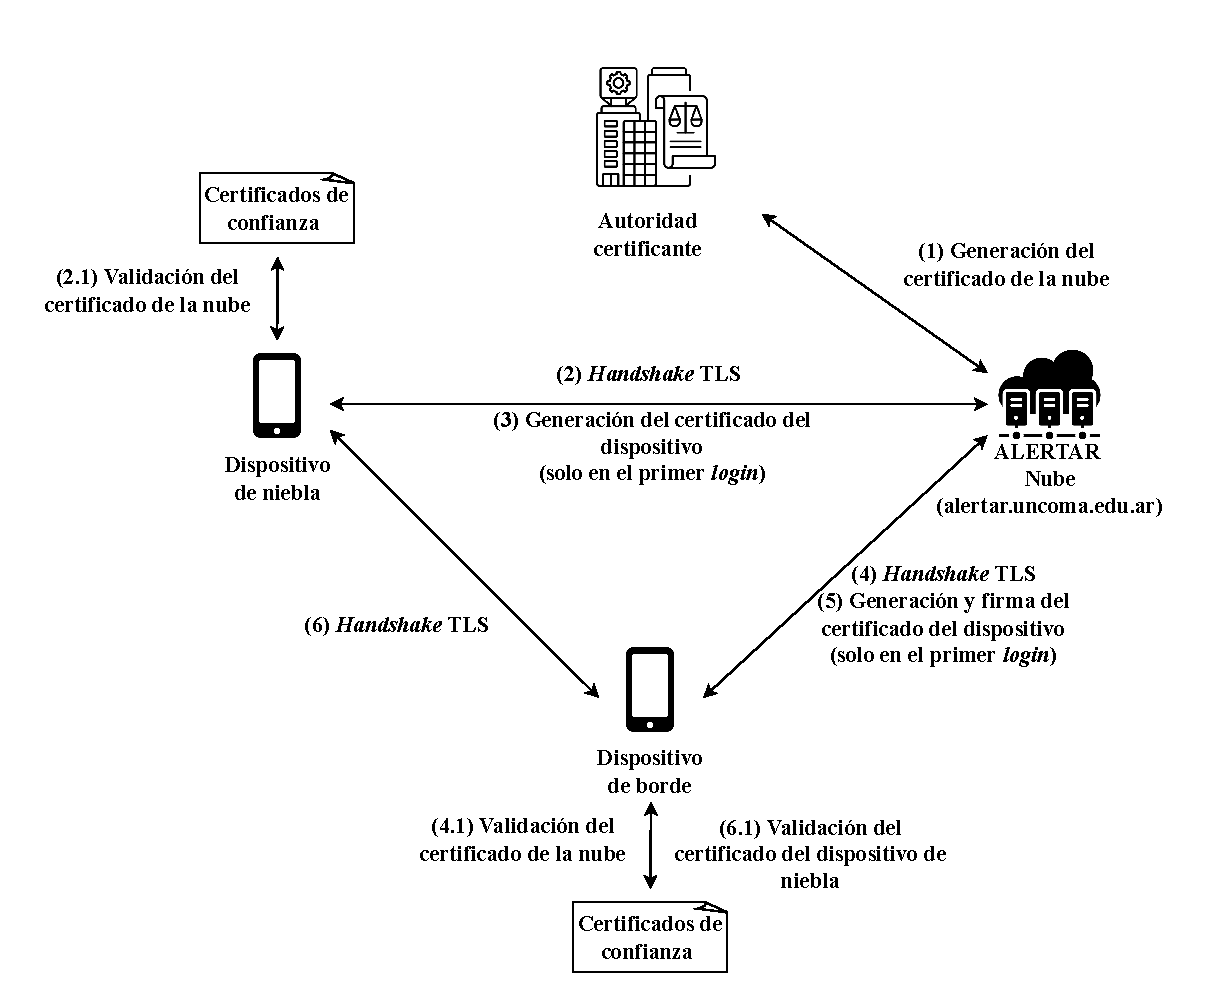
\includegraphics[width=\textwidth]{Imagenes/Implementacion/distribucionClaves.pdf}
    \caption{Generación, distribución y validación de certificados en el sistema ALERTAR}
    \label{fig:distClavesALERTAR}
\end{figure}

\section{Protocolo de comunicación}
\label{sec:protocoloComunicacion}
El sistema ALERTAR divide sus funcionalidades en casos de uso, la implementación de estos requiere del intercambio de información entre los componentes del sistema de las capas nube, niebla y de borde a través de mensajes. Con el propósito de permitir la interoperabilidad entre sistemas de cómputo heterogéneos, los mensajes se estructuran en formato JSON \cite{json_es} y se codifican utilizando el estándar UTF-8. Las operaciones se definen por el denominado \textit{protocolo de operaciones} y están definidas como:

\begin{itemize}
    \item \textit{\textbf{login: }}el usuario envía sus credenciales de identificación a un dispositivo de nivel de niebla o nube, según corresponda. Si la autenticación es exitosa, se responde con una lista de dominios (usuarios, hospitales y sectores) a los que el usuario puede suscribirse. Al finalizar, el dispositivo del usuario pasa a ser un dispositivo de borde.

    \item \textit{\textbf{data\_sync: }}luego de una autenticación exitosa, el dispositivo de borde sincroniza sus réplicas con las copias primarias de los dominios de su interés. Para esto, se envía un mensaje especificando, para cada dominio, el valor del reloj lógico más alto que tiene entre sus datos almacenados. Por cada dominio se reciben todos los datos que contengan un valor de reloj lógico mayor al especificado. Además, sólo en caso de estar sincronizado con la nube y no así con un dispositivo de niebla, se reciben los datos necesarios para establecer conexión con los dispositivos que mantienen las copias primarias de los dominios de interés. Por último, se realiza un cambio de conexión entre el dispositivo de borde y la nube, en caso de que exista, a una conexión entre el dispositivo de borde y el dispositivo de niebla a cargo del dominio de interés. Este procedimiento se detalla en la sección \ref{sec:autentic_seguridad}.

    \item \textit{\textbf{insert:}} es una petición de inserción de un nuevo dato al dispositivo que contiene la copia primaria del dominio. Verifica que no exista un registro con las mismas claves. Si la inserción es exitosa el dato se replica a través del método de \textit{copy}.

    \item \textit{\textbf{update:}} es una petición de modificación de un dato al dispositivo que contiene la copia primaria del dominio. A fin de mantener un registro histórico, la base de datos no modifica el registro original, sino que crea uno nuevo. Al insertar un nuevo registro, este tendrá un reloj lógico mayor al previo. Si existen varios registros con las mismas claves, el de mayor reloj lógico será el válido. Verifica que ya exista un registro con las mismas claves. Si la actualización es exitosa, el dato se replica a través del método \textit{copy}.

    \item \textit{\textbf{copy:}} cuando un dato es ingresado a la copia primaria, el dispositivo que la mantiene utiliza este mensaje para replicar el dato a todos los dispositivos que mantienen réplicas.


    \item \textit{\textbf{lead: }}es una solicitud a la nube para convertir dispositivos de borde en dispositivos de niebla. El usuario debe estar autorizado por la nube para realizar tal acción. Se debe especificar la dirección \textit{IP} y la clave pública del dispositivo. Esta información luego es utilizada para que los dispositivos de borde puedan intentar conectarse al de niebla a través de la red de área local.
\end{itemize}

La restricción para que funcione este protocolo es que una parte no puede enviar una nueva solicitud de operación hasta que la solicitud anterior haya sido resuelta.

En la Figura \ref{fig:secuenciaProtocolo} se detalla, a modo de ejemplo, un diagrama de secuencia donde se realiza un inicio de sesión, sincronización de datos e inserción de un nuevo paciente. Previo al inicio del ejemplo se considera que el cliente obtuvo la dirección del líder mediante un código QR o desde la nube:
\begin{enumerate}
    \item Un dispositivo de borde realiza una solicitud de \textit{login} al dispositivo de niebla a cargo del sector.
    
    \item Una vez recibida la solicitud el dispositivo de niebla prepara la respuesta \textit{infoUsuario} con información del usuario, así como los dominios a los cuales tiene permiso para suscribirse.
    
    \item Una vez recibida la respuesta al \textit{login}, el usuario procede a elegir uno o varios dominios para suscribirse. Luego se genera \textit{conjuntoDominios} el cual contiene el mayor valor de \textit{sync\_id} de cada dominio seleccionado. Finalmente, se realiza el envio en una solicitud de \textit{data\_sync} al dispositivo de niebla.

    \item Al recibir la solicitud de \textit{data\_sync}, el dispositivo de niebla, genera la respuesta \textit{datosDominios} a partir de los registros de cada dominio que tengan un \textit{sync\_id} mayor al especificado en la solicitud.

    \item El dispositivo de borde recibe los registros actualizados de sus dominios y actualiza su base de datos con estos.

    \item Al insertar un paciente, el dispositivo de borde solicita al usuario que ingrese los datos del paciente a ingresar. Una vez cargados estos datos se prepara \textit{datosPaciente} con ellos. Se envía una solicitud de inserción del paciente al dispositivo de niebla.

    \item Al recibir una solicitud de inserción el dispositivo de niebla realiza las validaciones correspondientes y, si está todo correcto, inserta un nuevo registro paciente en su base de datos local. Luego procede a realizar un proceso de \textit{copy} donde envía una solicitud con el nuevo registro a todos los dispositivos de borde suscritos al dominio que este dispositivo controla y a la nube en caso de tener conexión a ella.

    \item Todos los dispositivos de borde suscritos al dominio del sector operado, y la nube, reciben una solicitud de \textit{copy} para que guarden en su base de datos un nuevo registro
\end{enumerate}

Los pasos del uno al cinco se realizan una única vez por conexión, a la hora de establecerla. Los pasos del seis al ocho se realizan cada vez que se desea insertar un nuevo paciente.

\begin{figure}
    \centering
    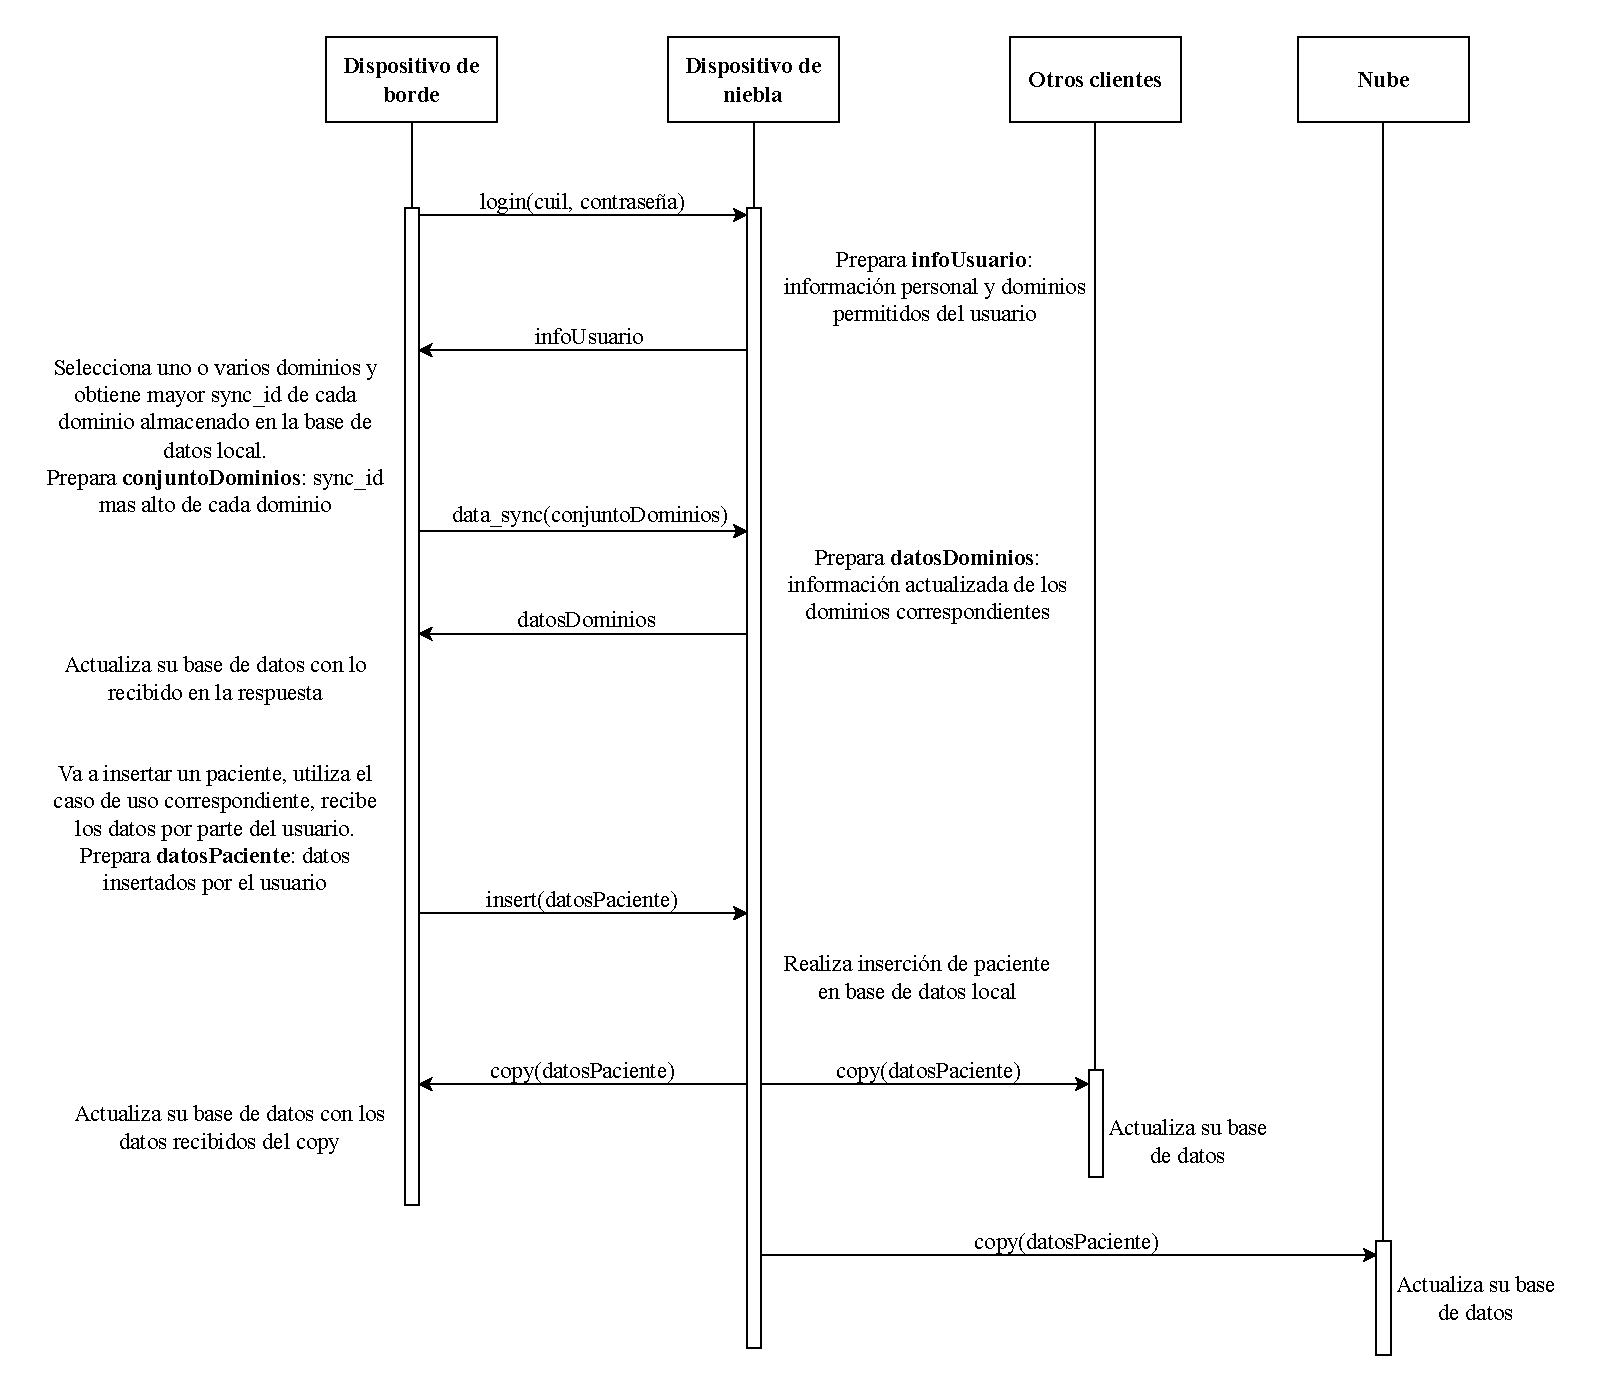
\includegraphics[width=\linewidth]{Imagenes/Implementacion/secuenciaProtocolo.pdf}
    \caption{Ejemplo de login, sincronización e inserción de paciente desde un dispositivo de borde.}
    \label{fig:secuenciaProtocolo}
\end{figure}

\section{Implementación de un manejador/gestor de mensajes discretos}
\label{sec:packageManager}
La aplicación ALERTAR requiere el envío y recepción de mensajes discretos. El protocolo TCP garantiza la entrega correcta y en orden de los datos al destinatario, pero no implementa el envío de los mensajes discretos. TCP puede particionar los mensajes en segmentos más pequeños durante la transmisión y luego re-ensamblarlos en el destino, pudiendo ocurrir que la cantidad de segmentos leídos en el destino no se corresponda con la cantidad de segmentos emitidos.

Por ejemplo, si un dispositivo de borde está conectado a un servidor y se envían los mensajes \texttt{Primer mensaje, Segundo mensaje,Tercer mensaje} de forma consecutiva, estos mensajes podrían enviarse en tres segmentos separados de la forma \texttt{[Primer mensaje], [Segundo mensaje], [Tercer mensaje]}. Alternativamente, los mensajes podrían agruparse en dos segmentos de la forma \texttt{[Primer mensajeSegun],[do mensajeTercer mensaje]}. Podrían enviarse todos juntos en un único segmento \texttt{[Primer mensaje\allowbreak Segundo mensaje\break Tercer mensaje]}. Por último, puede ocurrir que un único mensaje sea dividido en segmentos diferentes de la forma \texttt{[Pri], [me],[r mensaje]}.

Para lograr la implementación del envío de mensajes discretos se diseñó e implementó una biblioteca denominada TCP-package-manager. La biblioteca implementa un protocolo para el envío de mensajes que se define de la siguiente manera:

\paragraph{Lado del emisor:}
\begin{enumerate}
    \item Calcular la longitud del mensaje en bytes. Representar esta longitud como un entero sin signo de 4 bytes \textit{big-endian}. Por ejemplo, la longitud del mensaje \texttt{0x48 45 4C 4C 4F 20 57 4F 52 4C 44 21} se representa como \textit{0x00 00 00 0C}.
    \item Enviar la longitud calculada del mensaje.
    \item Enviar el mensaje original.
\end{enumerate}

\paragraph{Lado del receptor:}
\begin{enumerate}
    \item El receptor lee cuatro bytes del \textit{socket} de comunicaciones TLS/TCP.
    \item Interpretar los cuatro bytes leídos como la longitud del próximo mensaje, considerando que los bytes están en formato \textit{big-endian}.
    \item El receptor lee los $N$ bytes especificados en el paso anterior. Estos bytes contienen el mensaje original del emisor. En caso de que se reciba un segmento de menos de $N$ bytes se almacenan hasta que se logre completar los $N$ bytes especificados.
    
\end{enumerate}
El cálculo y envío de la longitud del mensaje original le permite al receptor saber cuántos bytes debe leer. Esto le permite leer correctamente los mensajes recibidos por más que estos no se envíen de forma discreta.

Realizando la conversión a \textit{big-endian} para el envío y su posterior interpretación en el lado del receptor, se asegura la correcta interpretación de los datos independientemente del dispositivo o arquitectura. Esto es importante ya que los procesadores pueden tener diferentes arquitecturas de \textit{endianness}, que determinan el orden en que se almacenan en memoria los bytes de datos multibyte, como enteros o flotantes.

\section{Mecanismo de detección de pérdida de conectividad}
\label{sec:perdidaConect}
Si bien el protocolo \textit{TCP} define mecanismos para la detección de fallos de conexión, la biblioteca utilizada para establecer comunicaciones \textit{TLS/TCP} presenta problemas para informarlos de manera apropiada e inmediata. Específicamente, cuando un dispositivo móvil pierde su conexión \textit{Wi-Fi} o de datos móviles, la biblioteca no logra detectar la desconexión. 

Para solucionar este problema, se implementó un protocolo de \textit{Heartbeat} y reconexión. En este protocolo, los dispositivos de borde envían un mensaje de \textit{``ping''} cada cierto tiempo. Una vez enviado el mensaje de \textit{``ping''}, los dispositivos de borde esperan una respuesta de \textit{``pong''} por parte del servidor, ya sea un dispositivo de niebla o la nube. La espera esta limitada a un tiempo $T$. Si $T$ expira, se considera que la conexión del dispositivo se ha cortado y se inicia un proceso de reconexión al líder. 

Si el servidor al que el dispositivo de borde está conectado es la nube, se consideran dos escenarios para la reconexión:

\begin{itemize}
    \item \textbf{Falla la nube: }Actualmente la nube no cuenta con reemplazo, pero cuando lo tenga se resolverá de manera transparente mediante \textit{DNS}. Los intentos de reconexión del protocolo son ilimitados. Es decir, se intentará reconectar a la nube hasta que se restablezca la conexión o se opte por conectarse manualmente a un dispositivo de niebla.
    \item \textbf{Falla la conectividad con la nube: }Los intentos de reconexión son ilimitados.
\end{itemize}

En el caso de que el servidor al que el dispositivo de borde estaba conectado se trate del dispositivo de niebla, como el problema de conexión puede deberse a un fallo del servidor, y el reemplazo no es transparente, luego de un determinado número de intentos se considera que la conexión se ha perdido de forma definitiva. En este caso, la aplicación inicia nuevamente la conexión al sistema, que comienza estableciendo contacto con la nube.

\begin{figure}
    \centering
    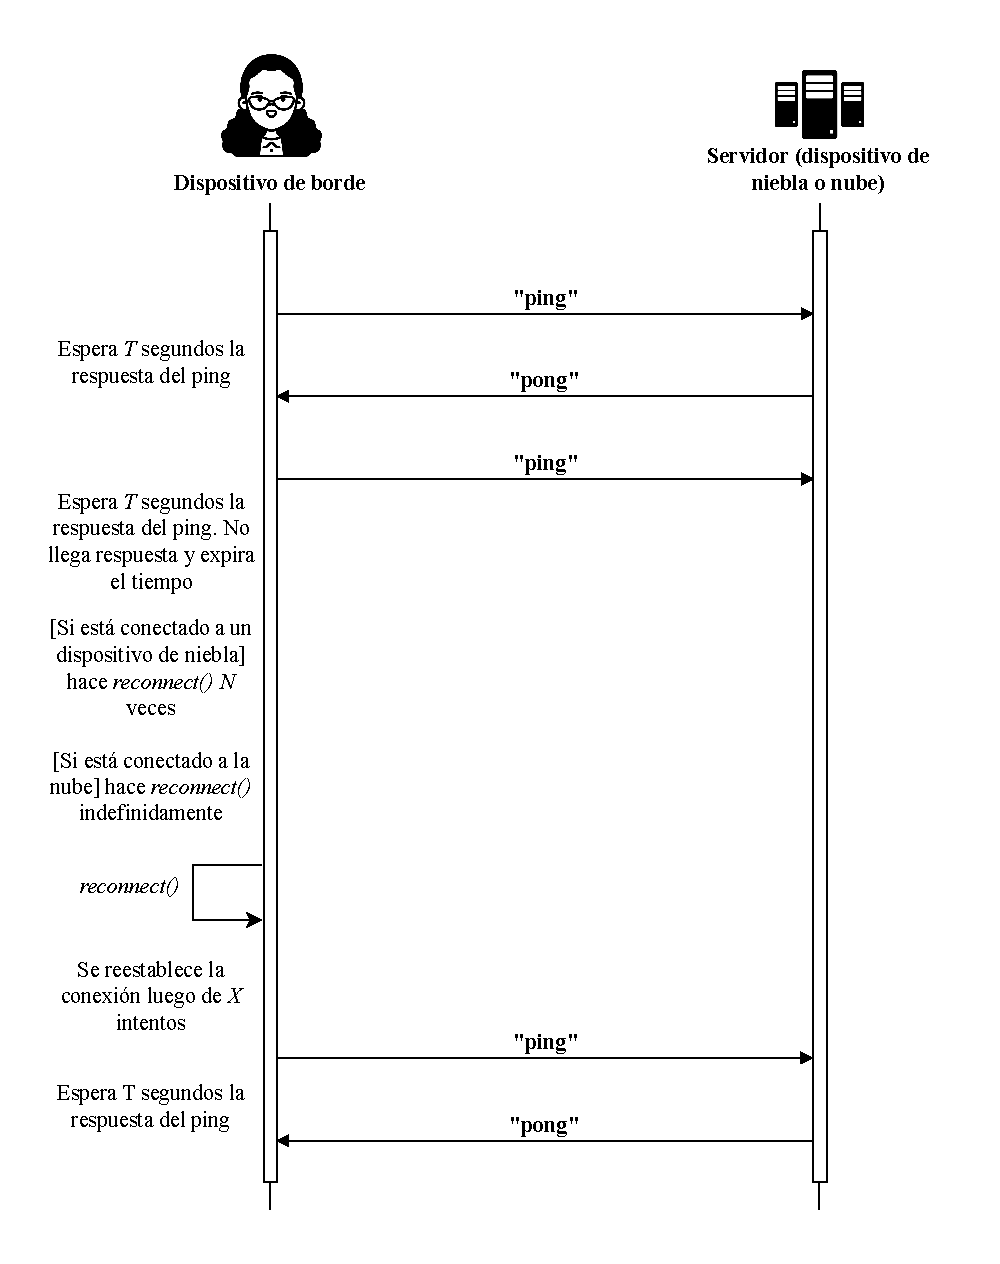
\includegraphics[width=14cm]{Imagenes/Implementacion/ProtocoloReconexion.pdf}
    \caption{Funcionamiento del protocolo de \textit{Ping} y reconexión ante fallos}
    \label{fig:protocoloReconexion}
\end{figure}


Al implementar este protocolo, los usuarios no deben preocuparse por la reconexión manual de los dispositivos, ya que el sistema se encarga automáticamente de detectar desconexiones y de restablecer la conexión ya existente sin necesidad de intervención del usuario. En caso de que no haya conectividad con la nube y el usuario desee cambiar la conexión a un nuevo dispositivo de niebla que se encuentre operativo, el proceso de conexión deberá realizarse de manera manual haciendo uso de un código \textit{QR} que se muestra en la pantalla del dispositivo de niebla al que se desea conectar.

En la figura \ref{fig:protocoloReconexion} se puede observar un ejemplo de su funcionamiento. En ella se asume que ya hay establecida una conexión previa entre un dispositivo de borde y un servidor nube o dispositivo de niebla. Se puede observar el intercambio de mensajes \textit{``ping''} y \textit{``pong''} entre las partes, cada vez que el dispositivo de borde envía un mensaje de \textit{``ping''} espera un tiempo $T$ a que el servidor le responda con un \textit{``pong''}. En caso de que el tiempo $T$ expire se considera que hubo una pérdida de conexión, en cuyo caso se plantean dos posibles escenarios:
\begin{itemize}
    \item El dispositivo de borde está conectado a un dispositivo de niebla: Se procede a realizar los $N$ intentos de reconexión haciendo uso de \textit{reconnect()}.
    \item El dispositivo de borde está conectado a la nube: Se procede a realizar intentos de reconexión de manera indefinida con \textit{reconnect()}.
\end{itemize}

Una vez restablecida la conexión se reanuda el intercambio de mensajes entre las partes.





\section{Serialización de las operaciones}
\label{sec:serializacion}
Para evitar la aparición de errores o estados inconsistentes en los dispositivos y mantener la consistencia del sistema, es crucial garantizar que las operaciones sean procesadas en el mismo orden en el que son recibidos los mensajes que las accionan.

Para comprender qué ocurre ante la inexistencia de serialización, se plantea el siguiente escenario como ejemplo: un dispositivo de borde recibe dos peticiones de \textit{copy} por parte del dispositivo de niebla. La primera tiene un registro paciente con $sync\_id=4$ y la segunda un registro paciente $sync\_id=5$. Se asume que las operaciones en el dispositivo de borde no están serializadas. El guardado del registro con $sync\_id=5$ finaliza antes que el del registro con $sync\_id=4$. Si el dispositivo llegara a tener un fallo que impidiera finalizar la inserción del registro con $sync\_id=4$, al realizar el proceso de \textit{data\_sync} se enviará el valor de $sync\_id=5$, ya que es el más alto del dominio sector en la base de datos local del dispositivo de borde. Esto produce que el registro con $sync\_id=4$ no se vuelva a sincronizar nunca lo cual provoca la pérdida de dicho dato en la réplica del dominio sector del dispositivo de borde.

\textit{TypeScrypt} es un sistema basado en eventos con un único hilo. Para gestionar y coordinar las operaciones asíncronas, de manera que puedan ejecutarse de manera eficiente sin bloquear el hilo principal, \textit{TypeScrypt} usa el denominado \textit{event loop}\cite{ecma262}. En este, si por ejemplo, se tienen tres funciones asíncronas: \textit{validate()}, \textit{updateDataSync()}, e \textit{insert()}, y no se utiliza un mecanismo de sincronización, las funciones pueden empezar a ser ejecutadas sin esperar a que las tareas previas terminen.

Para controlar el orden de ejecución de las llamadas, TypeScript utiliza dos estructuras principales: la pila de ejecución y la cola de tareas. La pila de ejecución \textit{(stack)} es una estructura que gestiona la ejecución de funciones según el orden en que se llaman. Cuando una función es invocada, se añade a la pila y comienza su ejecución pausando la ejecución de su llamador. Si esa función llama a otra, esta nueva función también se añade a la pila y se continúa con la ejecución de esta, pausando la ejecución de la llamadora, así sucesivamente. Una vez que una función completa su ejecución, se elimina de la pila, y el control vuelve a la función anterior. Este proceso continúa hasta que la pila esté vacía, permitiendo que siga un flujo de ejecución organizado permitiendo invocaciones anidadas y recursión.

Por otro lado, al utilizar funciones asíncronas, se lanzan tareas no bloqueantes, las cuales no necesariamente son aquellas delegadas a componentes externos del sistema, que se colocan en una cola de tareas. El \textit{event loop} se encarga de gestionar estas tareas, ejecutándose cuando la pila de ejecución está vacía.

Entonces, volviendo al ejemplo donde se ejecutan \textit{validate()}, \textit{updateDataSync()}, e \textit{insert()}, cuando cualquiera de estas funciones llegue a una operación asíncrona (como una promesa\footnote{Una promesa es un objeto que representa la eventual resolución o rechazo de una operación asíncrona, permitiendo manejar su resultado en el futuro a través de métodos como \textit{.then()} o \textit{await}.} o una operación de entrada/salida (I/O)), esa tarea, que corresponde a la ejecución de la operación, se envía a la cola de tareas (En realidad TypeScript cuenta con dos colas, una de microtareas y otra de macro tareas). No se bloquea la ejecución esperando el resultado de la tarea, simplemente se continúa con la ejecución de la siguiente línea de código que corresponda. Luego, el \textit{event loop} revisa la cola de tareas y las ejecuta cuando la pila de llamadas esté vacía.

Al aplicar el mecanismo de sincronización mediante await, la pila de llamadas se detiene temporalmente en esa línea de código, esperando a que la promesa se resuelva. Una vez que la promesa se resuelve, la ejecución de la función continúa, y finalmente, cuando termina, la función se retira de la pila de llamadas. De esta manera, se garantiza la serialización de las operaciones asíncronas, ya que estas se van a ejecutar de manera secuencial y en el orden definido por el programa.

En la Figura \ref{fig:ejemploEventLoop} se puede observar un ejemplo, asumiendo que las funciones están dentro de un método \textit{main()} que se muestra en la Figura \ref{fig:eventLoopCodigo}. En la mitad izquierda de la sub figura \ref{fig:eventLoop}, la cual representa las llamadas sin el mecanismo de sincronización await, se tendrá el siguiente comportamiento:

\begin{enumerate} 
    \item \textbf{Llamada a \textit{main()}} $\rightarrow$ main() sube a la pila de llamadas.
    
    \item \textbf{Llamada a validate()} $\rightarrow$ validate() sube a la pila de llamadas. Se crea una promesa que se retorna inmediatamente y la tarea relacionada a esa promesa se envía a la cola de tareas. 
    
    \item \textbf{validate() termina} $\rightarrow$ La parte síncrona de validate() se ejecuta, y luego validate() sale de la pila de llamadas. 
    
    \item \textbf{Llamada a updateDataSync()} $\rightarrow$ updateDataSync() sube a la pila de llamadas. Se crea una promesa que se retorna inmediatamente y su resolución se guarda en la cola de tareas. 
    
    \item \textbf{updateDataSync() termina} $\rightarrow$ La parte síncrona de updateDataSync() se ejecuta, y luego updateDataSync() sale de la pila de llamadas. 
    
    \item \textbf{Llamada a insertPaciente()} $\rightarrow$ insertPaciente() sube a la pila de llamadas. Se crea una promesa que se retorna inmediatamente y la tarea correspondiente se encola para su posterior ejecución.

 \item \textbf{insertPaciente() termina} $\rightarrow$ La parte síncrona de insertPaciente() se ejecuta, y luego insertPaciente() sale de la pila de llamadas. 
    
    \item \textbf{El \textit{event loop} gestiona la cola de tareas} $\rightarrow$ Después de que la pila de llamadas esté vacía, el \textit{event} loop procesa las promesas pendientes de resolución en la cola de tareas. 
\end{enumerate}

En este caso el llamador no espera la finalización de las funciones asíncronas para continuar con su ejecución. Es decir, no se aplica ningún mecanismo de sincronización.

Para la segunda parte de la Figura \ref{fig:eventLoop}, donde sí se hace uso de \textit{await}, el método de sincronización hace una espera para que finalice cada llamada antes de continuar con la ejecución que se encuentra después de ella:

\begin{enumerate}
    \item \textbf{Llamada a \textit{main()}} $\rightarrow$ \textit{main()} sube a la pila de llamadas. Se ejecuta hasta el primer \textit{await}.
    
    \item \textbf{\textit{await validate()}} $\rightarrow$ \textit{main()} se pausa en \textit{validate()} hasta que la promesa se resuelva en la cola de tareas.
    
    \item \textbf{Resolución de \textit{validate()}} $\rightarrow$ La promesa de \textit{validate()} se resuelve, \textit{main()} se reanuda y continúa con \textit{updateDataSync()}.
    
    \item \textbf{\textit{await updateDataSync()}} $\rightarrow$ \textit{main()} se pausa en \textit{updateDataSync()} hasta que la promesa se resuelva en la cola de tareas.
    
    \item \textbf{Resolución de \textit{updateDataSync()}} $\rightarrow$ La promesa de \textit{updateDataSync()} se resuelve, \textit{main()} se reanuda y continúa con \textit{insertPaciente()}.
    
    \item \textbf{\textit{await insertPaciente()}} $\rightarrow$ \textit{main()} se pausa en \textit{insertPaciente()} hasta que la promesa se resuelva en la cola de tareas.
    
    \item \textbf{Resolución de \textit{insertPaciente()}} $\rightarrow$ La promesa de \textit{insertPaciente()} se resuelve, \textit{main()} se reanuda y finalmente termina, saliendo de la pila de llamadas.
\end{enumerate}

De esta manera, al utilizar \textit{await} en cada función asíncrona, el event \textit{loop} se encarga de pausar la ejecución de \textit{main()} hasta que cada promesa se resuelva. Esto asegura que las operaciones se ejecuten de forma secuencial, respetando el orden de las llamadas. Gracias al \textit{await}, se garantiza la ejecución secuencial de las operaciones.

\begin{figure}[]
    \centering    
    \begin{subfigure}{\textwidth}
        \centering 
        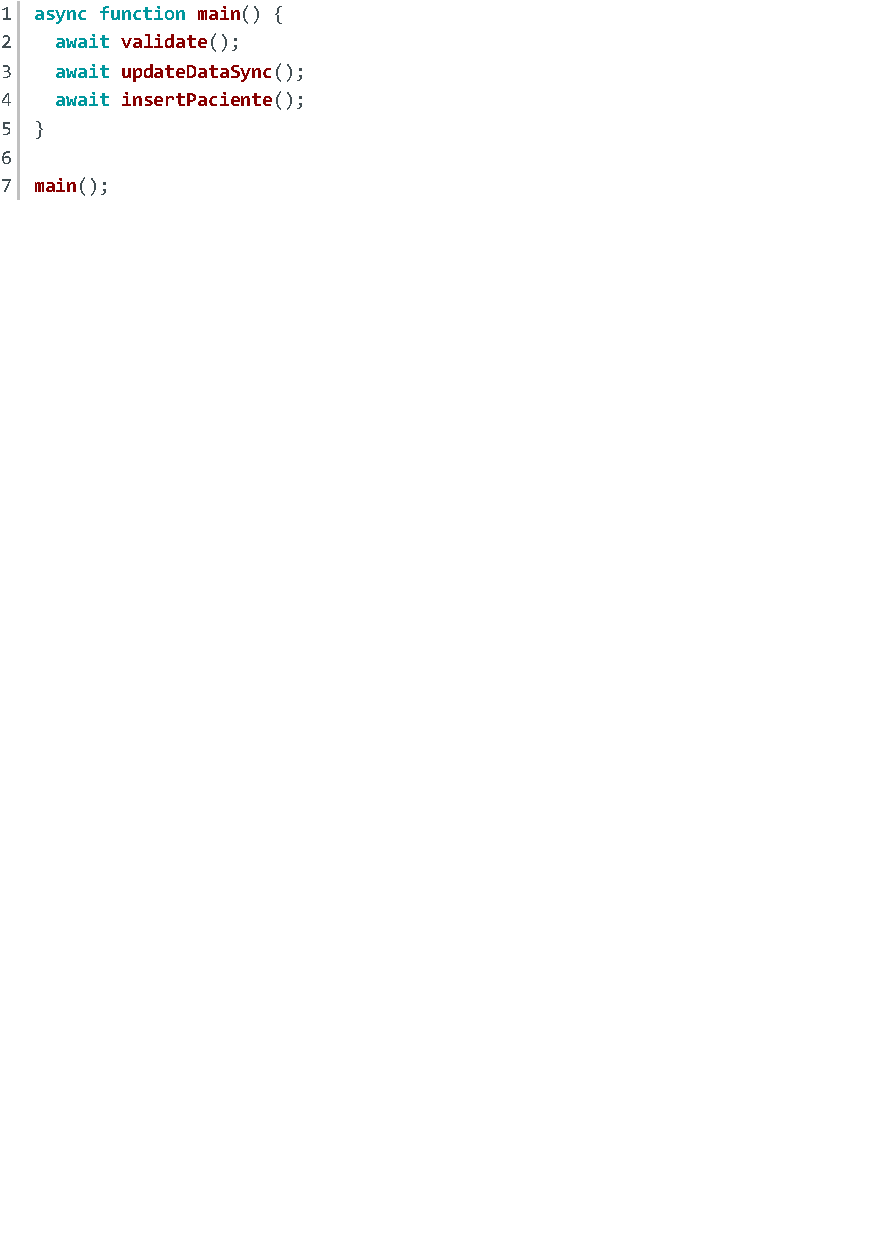
\includegraphics[width=0.5\textwidth]{Imagenes/Implementacion/eventLoopCodigo.pdf}
        \caption{Función main() contiene a las tres funciones}
        \label{fig:eventLoopCodigo}
    \end{subfigure}
    \begin{subfigure}{\textwidth}
        \centering 
        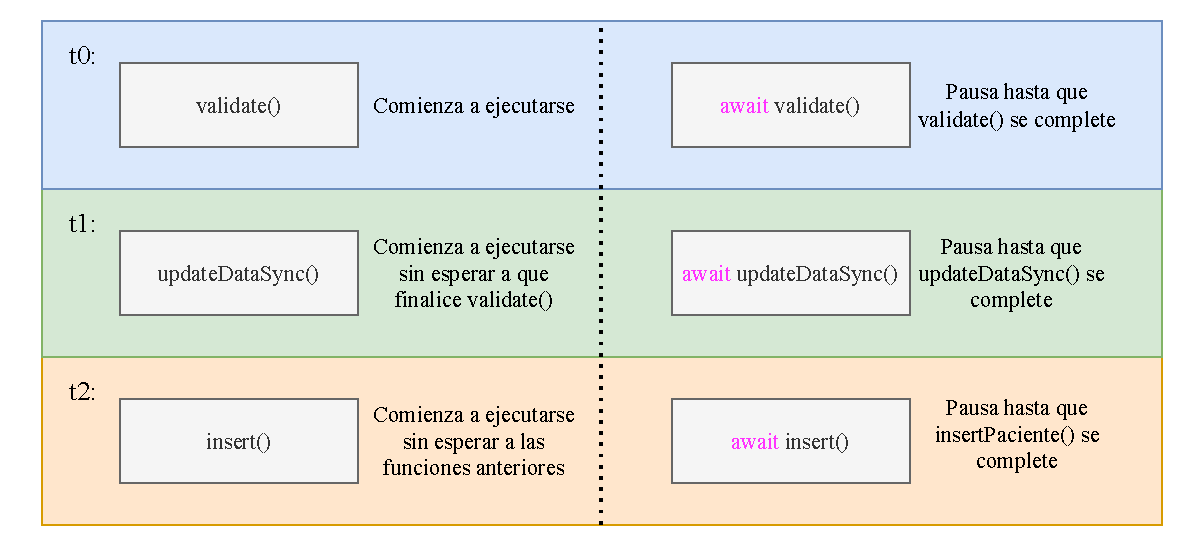
\includegraphics[width=\textwidth]{Imagenes/Implementacion/eventLoop.pdf}
        \caption{Secuencia y tiempos de llamadas del event loop}
        \label{fig:eventLoop}
    \end{subfigure}
    \caption{Ejemplo de comportamiento de event loop}
    \label{fig:ejemploEventLoop}
\end{figure}

\section{Diseño arquitectónico y especificaciones de la implementación}
\label{sec:implementacion}
La implementación del núcleo del sistema ALERTAR consiste en dos aspectos clave, los casos de uso y los servicios para los dispositivos de borde y niebla. Ambos aspectos fueron diseñados e implementados haciendo uso de una arquitectura limpia.

\subsection{Implementación de la arquitectura limpia}
Se implementaron tres capas que constituyen la arquitectura limpia del núcleo de la aplicación móvil ALERTAR. Estas se encuentran detalladas en la Figura \ref{fig:capasArquitectura} donde se puede observar, representadas con flechas, las dependencias de las capas de \textit{interfaz de usuario} y \textit{datos} con la capa de \textit{dominio}. De esta manera, se logra que los componentes de la capa de dominio sean independientes de implementaciones concretas de interfaces gráficas, bases de datos, servicios y repositorios. Las capas se definen de la siguiente manera:

\begin{itemize}
    \item \textbf{Interfaz de usuario: }Aquí se definen las interfaces a través de las cuales los usuarios interactúan con el sistema, en este caso las vistas y componentes interactivos de la aplicación móvil.
    
    \item \textbf{Dominio: }Aquí se definen los \textit{casos de uso} los cuales determinan las funcionalidades a las cuales pueden acceder los usuarios. Las \textit{entidades}, las cuales son objetos que contienen datos junto con las funciones que los manipulan, son independientes de cualquier infraestructura por lo que pueden ser utilizadas por cualquier capa de la aplicación. Por último, las \textit{interfaces de repositorios} que determinan cómo es que interactúa la capa de dominio con la capa de datos. Estas interfaces garantizan que la capa de dominio permanezca aislada e independiente de implementaciones específicas, las cuales son delegadas a la capa de datos.

    \item \textbf{Datos: }Aquí se realizan las implementaciones de los repositorios, se definen las interfaces de bases de datos y servicios, junto con sus implementaciones concretas.
\end{itemize}

\begin{figure}
    \centering
    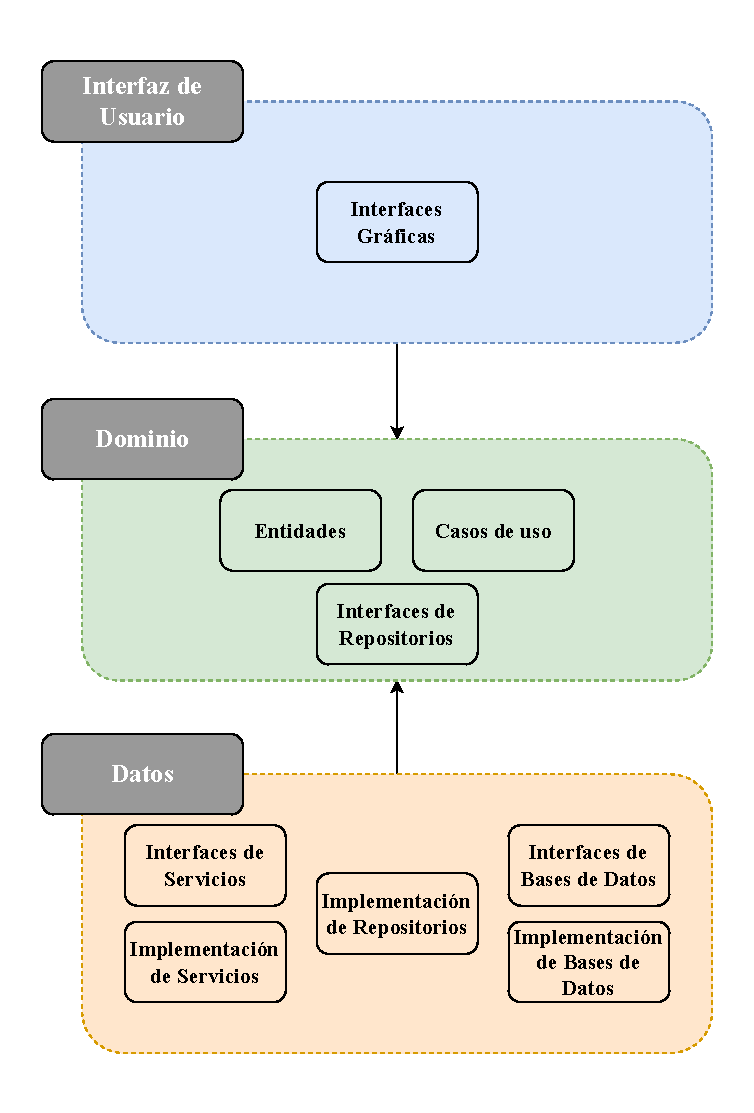
\includegraphics[width=0.7\linewidth]{Imagenes/Implementacion/CapasArquitectura.pdf}
    \caption{Arquitectura limpia del núcleo de la aplicación móvil del sistema ALERTAR}
    \label{fig:capasArquitectura}
\end{figure}
La forma en la cual interactúan entre sí las diferentes capas de la arquitectura limpia implementada se representa en la Figura \ref{fig:comunCapasArquitectura}. En ésta, los usuarios ejecutan casos de uso a través de una interfaz gráfica correspondiente a la capa de \textit{interfaz de usuario}. Los casos de uso, correspondientes a la capa de \textit{dominio}, utilizan interfaces de repositorios y entidades para definir su funcionalidad. Las implementaciones de las interfaces de los repositorios se envían a través del constructor del caso de uso. Las implementaciones de los repositorios corresponden a la capa de \textit{datos}. Por último, las clases concretas que implementan los repositorios utilizan interfaces de bases de datos y servicios, lo que las hace independientes de sus implementaciones específicas. Por ejemplo, si se quisiera cambiar el tipo de base de datos de relacional a no relacional, no sería necesario modificar la lógica del repositorio, ya que utiliza una interfaz para acceder a su fuente de datos, en lugar de depender de una implementación específica.

Además, se observa que los servicios interactúan directamente con los casos de uso, dado que las solicitudes realizadas por los dispositivos de borde hacia los de niebla requieren ser resueltas mediante la ejecución de dichos casos de uso. La recepción y cómputo de los mensajes se realiza a través de los servicios, lo que implica que estos deben invocar los casos de uso correspondientes para procesar y responder adecuadamente a las peticiones recibidas.
\begin{figure}
    \centering
    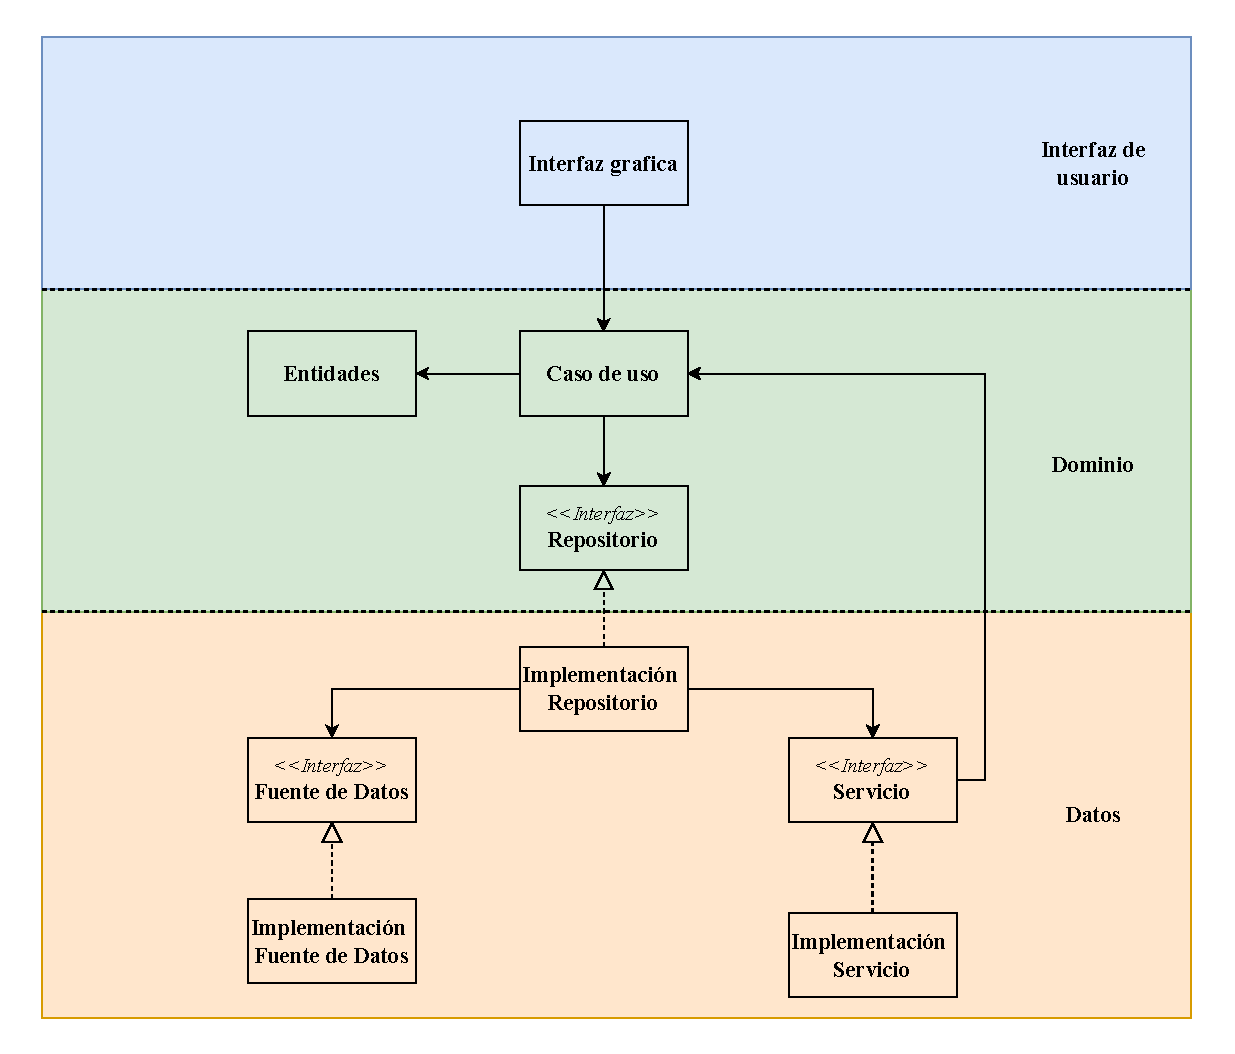
\includegraphics[width=1\linewidth]{Imagenes/Implementacion/ComunicacionCapas.pdf}
    \caption{Comunicación entre las capas de la arquitectura limpia}
    \label{fig:comunCapasArquitectura}
\end{figure}

Aplicando esta arquitectura se logra que los diferentes componentes de la aplicación puedan evolucionar o ser modificados de manera independiente. Lo que permite que el sistema sea modular, mantenible y flexible.

\subsection{Servicios de los dispositivos de borde y niebla}
Dado que los dispositivos de niebla deben actuar como servidores, se definió una interfaz denominada \texttt{LiderService}, que agrupa todas las operaciones necesarias para su gestión. Esta interfaz se ilustra en la Figura \ref{fig:liderService} y define cómo debe crearse el servidor en los dispositivos, delegando la responsabilidad a la clase \texttt{Server}. Para abstraer el tipo de protocolo de transporte utilizado, se adoptó el patrón \textit{Factory} mediante la interfaz \texttt{ConnectionFactory}, lo que permite implementar e instanciar diferentes tipos de conexión para el servidor en caso de ser necesario.


Entre las operaciones que define \texttt{LiderService} se incluyen: la creación del servidor, el manejo de nuevas conexiones, el envío de réplicas a todos los dispositivos conectados (\textit{copy}) y la recepción de mensajes discretos. Para estas últimas dos tareas, se hace uso de la clase \texttt{PackageManager}.

Una vez decodificado un mensaje por parte de un dispositivo de niebla, se determina y ejecuta el caso de uso correspondiente. Esta dependencia hacia los casos de uso se representa de manera simplificada en la Figura \ref{fig:liderService} con la clase \texttt{CasosDeUso}, la cual representa a todos los casos de uso. La clase \texttt{LiderServiceImpl}, que implementa la interfaz \texttt{LiderService}, es responsable de procesar la petición, enviar la respuesta al dispositivo de borde que la originó y propagar el \textit{copy} resultante tanto a la nube como al resto de los dispositivos de borde conectados.




\begin{figure}
    \centering
    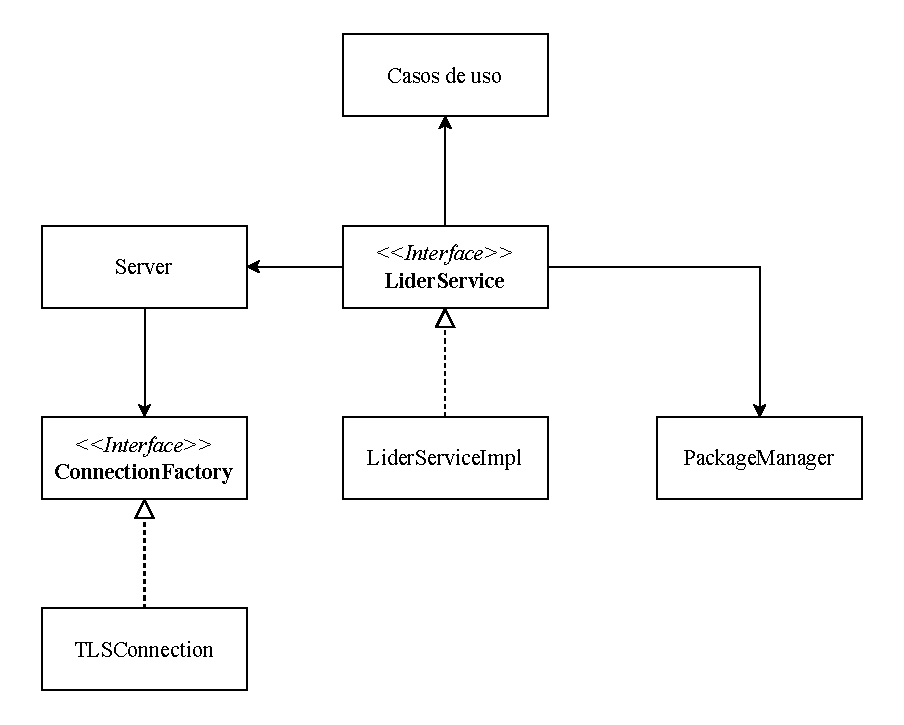
\includegraphics[width=\linewidth]{Imagenes/Implementacion/LiderService.pdf}
    \caption{Servicio de los dispositivos de niebla}
    \label{fig:liderService}
\end{figure}

Por otro lado, todos los dispositivos de borde deben conectarse a un servidor, ya sea la nube o un dispositivo de niebla. Para esto, se definió una interfaz denominada \texttt{UserService}, ilustrada en la Figura \ref{fig:clientService}. Esta interfaz, agrupa las operaciones necesarias para establecer y mantener la conexión de los dispositivos con el servidor, incluyendo: conexión, desconexión, reconexión y el envío y recepción de mensajes con el servidor. Al igual que \texttt{LiderService}, los detalles de la gestión de conexión, como por ejemplo la creación y manejo de \textit{sockets} con el servidor, se delega en la clase \texttt{Server}.

Tal como se observa en la figura \ref{fig:clientService}, \texttt{UserService} hace uso de la clase \texttt{PackageManager} para garantizar que los mensajes se transmitan como unidades discretas. La clase \texttt{PingService} es responsable de implementar el protocolo de \textit{heartbeat}, utilizado para detectar interrupciones en la conectividad y disparar los mecanismos de reconexión cuando sea necesario. Además, se necesita poder ejecutar el caso de uso de inicio de sesión para poder gestionar reconexiones de manera completa. Para esto, utiliza la clase \texttt{UserLoginUseCase}.


Por último, se debe considerar que, como todos los dispositivos se conectan al servidor a través de \texttt{UserService}. De este modo, todos los mensajes provenientes del servidor son procesados por esta clase. En caso de que un mensaje recibido requiera funcionalidad específica del rol de niebla del dispositivo, entonces \texttt{UserService} delega el manejo de dicha funcionalidad a \texttt{LiderService}.


\begin{figure}
    \centering
    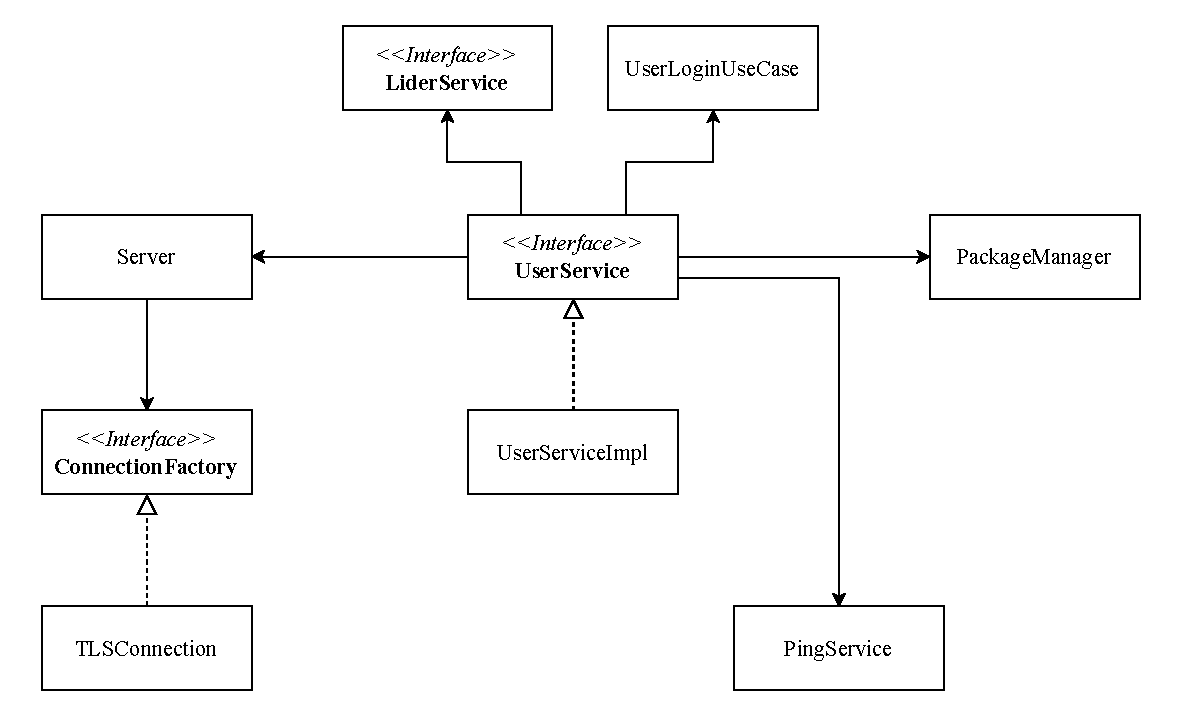
\includegraphics[width=\linewidth]{Imagenes/Implementacion/UserService.pdf}
    \caption{Servicio de los dispositivos de borde}
    \label{fig:clientService}
\end{figure}

\subsection{Casos de uso}
Los casos de uso son aquellas funcionalidades a las cuales el personal del hospital tiene acceso a través de la aplicación móvil, estan representados en el diagrama de la Figura \ref{fig:diagCasosUso} donde las flechas indican una dependencia unidireccional entre las capas. A continuación se detalla el objetivo de cada caso de uso:

\begin{itemize}
    \item \textbf{Iniciar sesión: }Valida el CUIL y contraseña del usuario para poder comenzar a utilizar la aplicación móvil. Como respuesta devuelve la información del usuario y los dominios a los cuales puede conectarse.
    \item \textbf{Conectarse a dominio:} El usuario selecciona el dominio al cual desea conectarse, como resultado se sincroniza toda la información de dicho dominio en el dispositivo móvil del usuario.
    \item \textbf{Admisión de paciente:} El usuario carga la información del paciente al ingresar. Esta operación es enviada a través de una solicitud y computada por un dispositivo de niebla. Finalmente, el dispositivo de borde del usuario, recibe una réplica por parte del dispositivo de niebla. La actualización de los pacientes es una variante de este mismo caso de uso.
    \item \textbf{Convertir a dispositivo de niebla:} El usuario convierte su dispositivo de borde a uno de niebla. Para poder hacerlo el usuario debe ser de tipo ``Jefe de enfermería'' o ``Jefe de clínica médica''
    \item \textbf{Asignar cama: }El usuario asigna un nuevo estado para una cama, es decir indica si se encuentra ocupada, desocupada o inhabilitada.
    \item \textbf{Modificar datos personales paciente: }Modifica los datos personales de un paciente ya ingresado.
    \item \textbf{Ver ficha de paciente: }Muestra la lista de fichas de todos los pacientes ingresados, permitiendo buscar una en especifico y leerla en detalle. 
    \item \textbf{Ver estado camas: }Muestra el estado de todas las camas del dominio seleccionado.
\end{itemize}

\begin{figure}
    \centering
    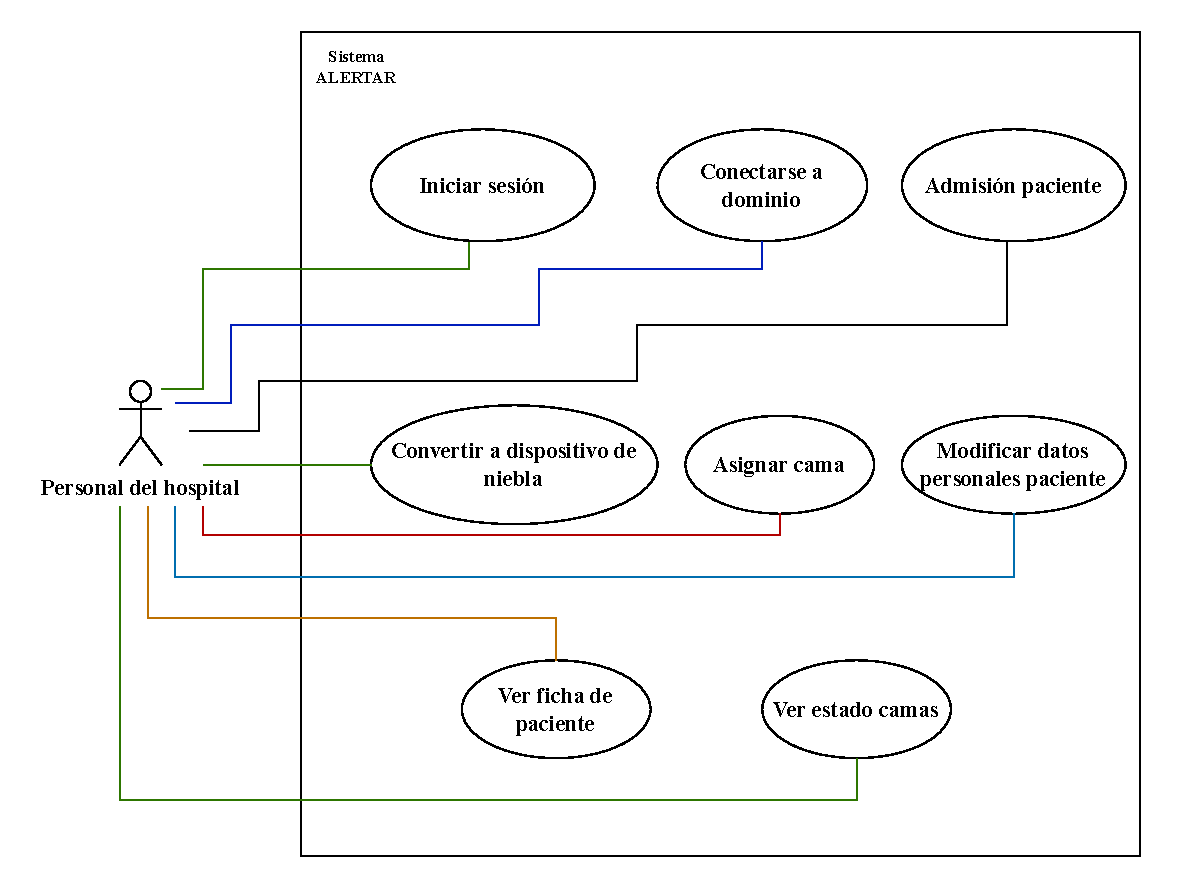
\includegraphics[width=\textwidth,keepaspectratio]{Imagenes/Implementacion/CasosDeUso.pdf}
    \caption{Diagrama de casos de uso de la aplicación móvil ALERTAR}
    \label{fig:diagCasosUso}
\end{figure}


Un diagrama de actividades del caso de uso \textit{Admisión paciente} se detalla en la Figura \ref{fig:diagActAdmPaciente}. En esta, se puede observar cómo cada conjunto de actividades se corresponde a una capa de la arquitectura limpia diseñada. El ingreso de los datos de un paciente y las notificaciones de fallo y éxito se corresponden a la capa de \textit{Interfaz de usuario}, enmarcadas en azul. La generación de la petición para computar el caso de uso, por parte del dispositivo de borde, y la validación de los datos de esta por parte del dispositivo de niebla se corresponden a la capa de \textit{Dominio}, encuadradas en verde. Por último, la creación y almacenamiento de un nuevo registro ``Paciente'' en ambos dispositivos, y la réplica del registro por parte del dispositivo de borde, corresponden a la capa de \textit{Datos}, enmarcada en amarillo.

\begin{figure}
    \centering
    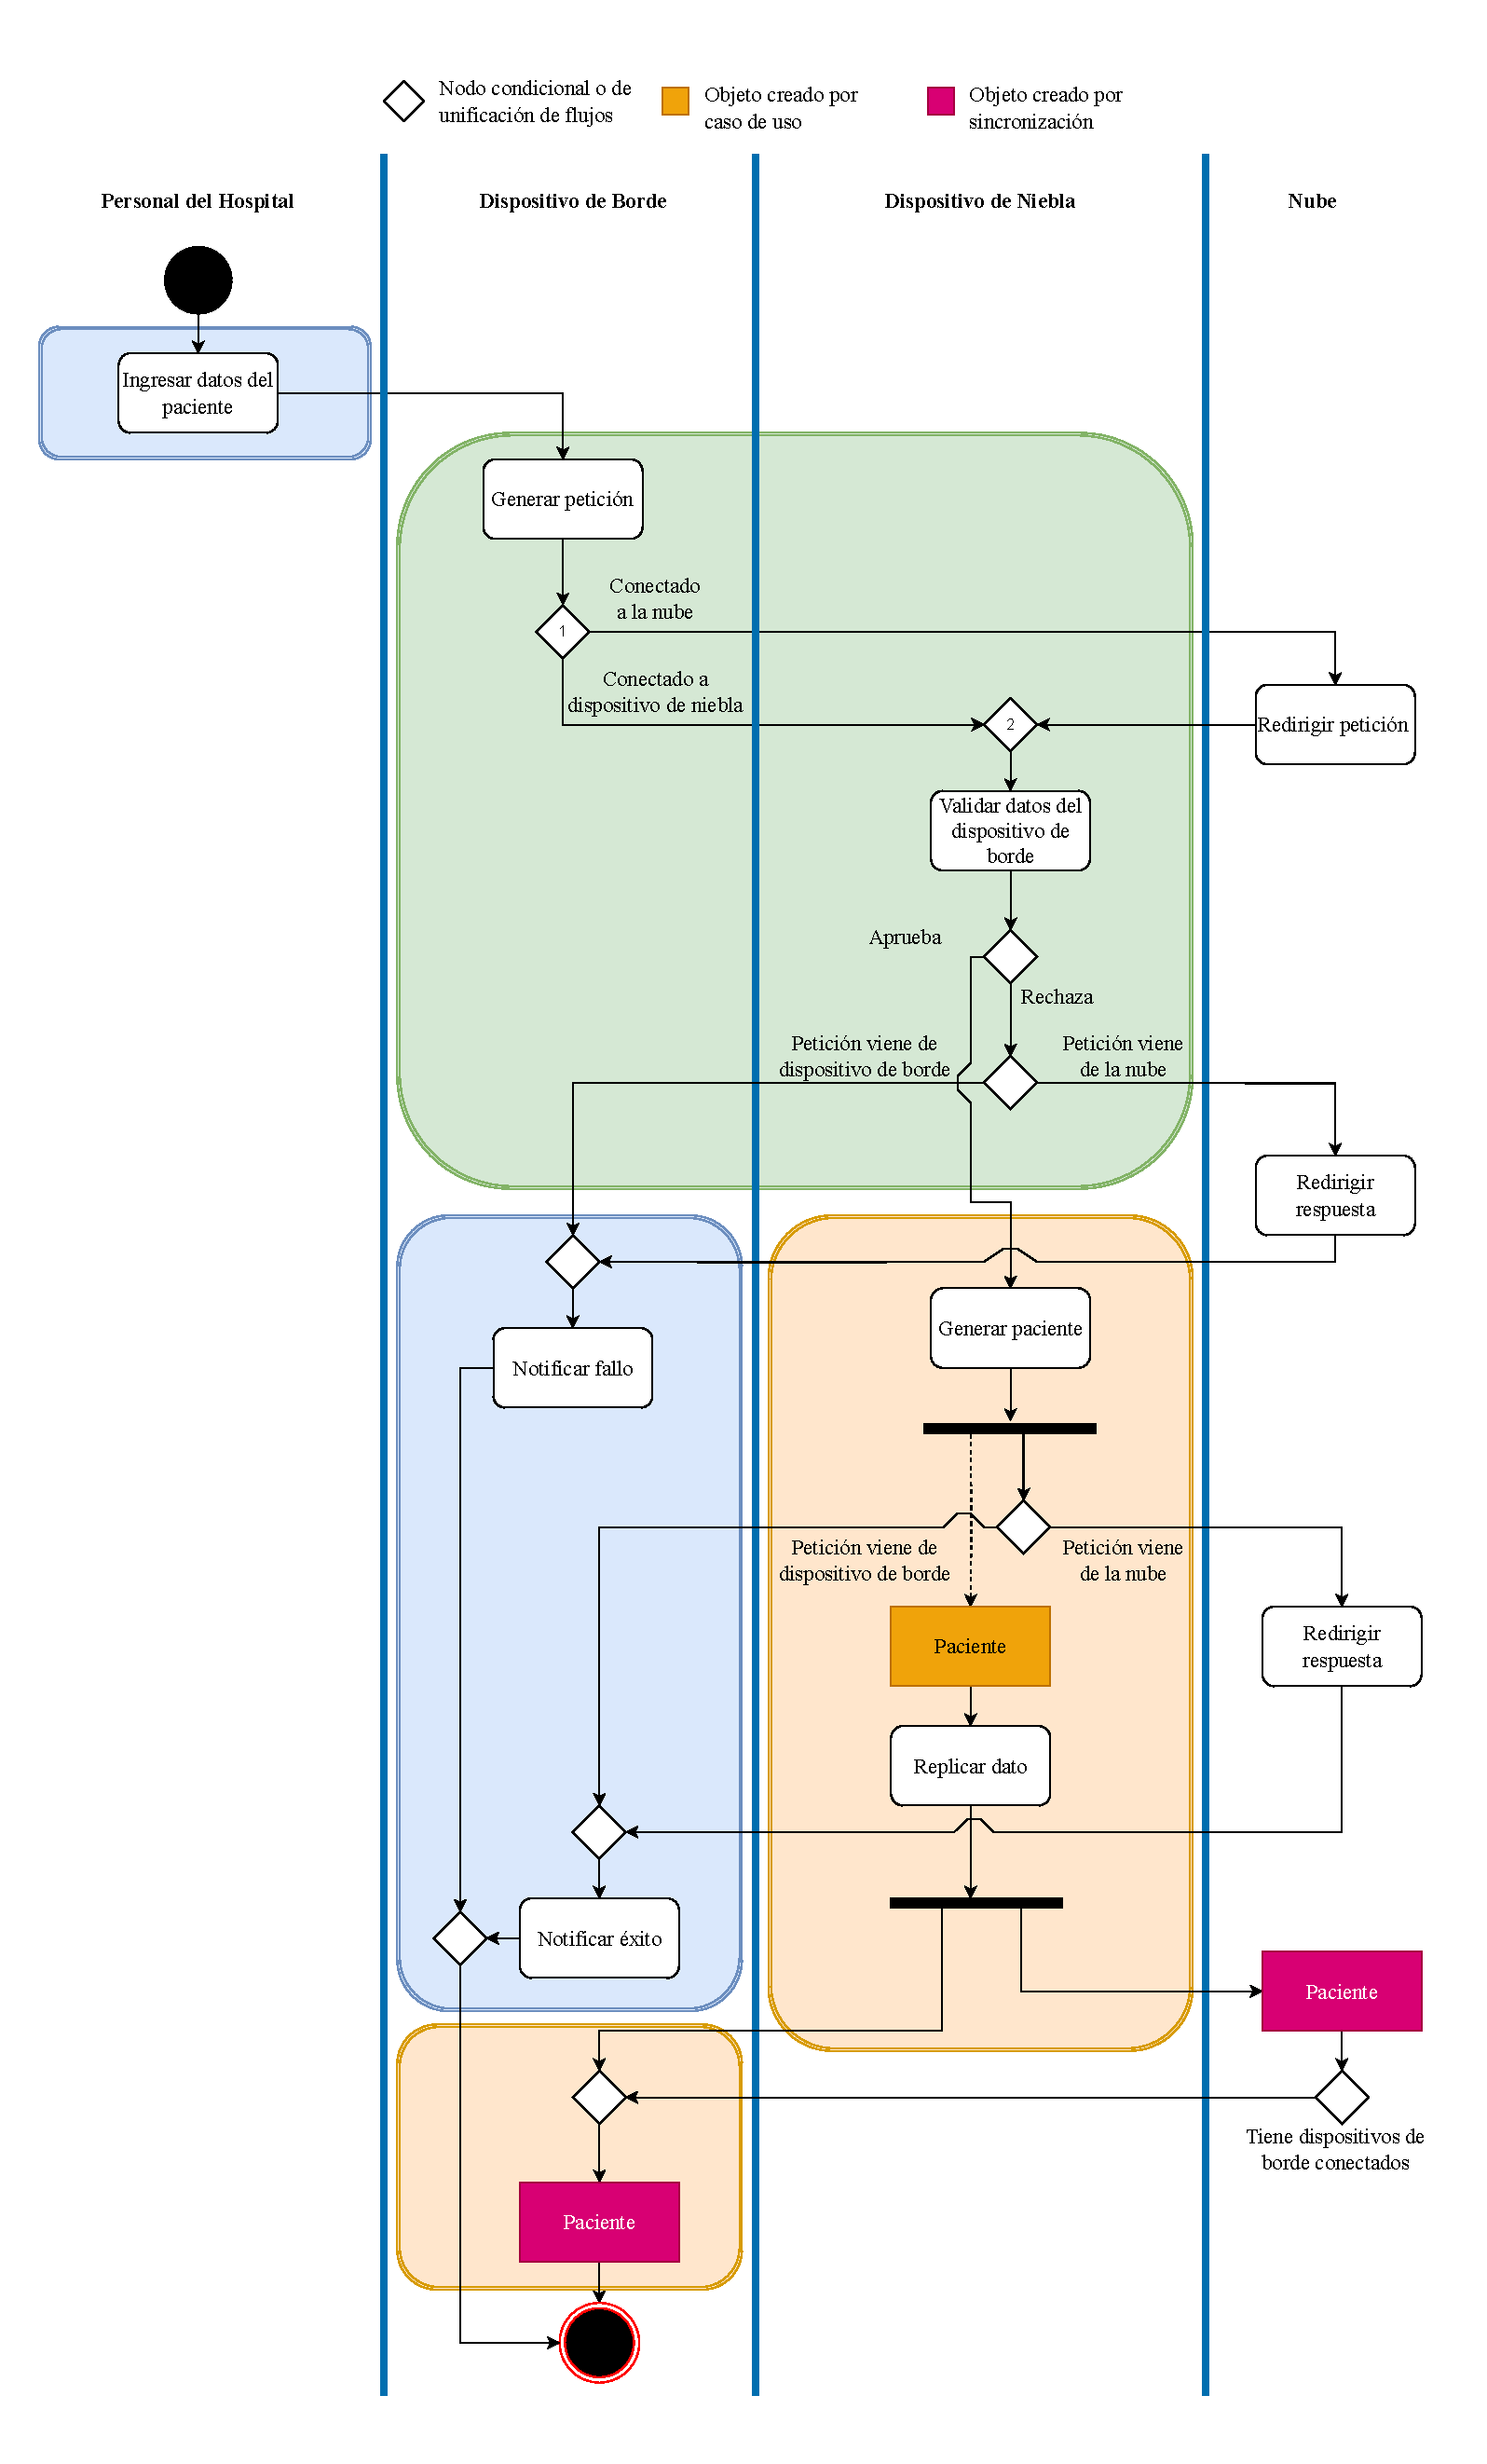
\includegraphics[width=\textwidth, height=\textheight, keepaspectratio]{Imagenes/Implementacion/DetalladoIngresarPaciente.pdf}
    \caption{Diagrama de actividades del caso de uso \textit{Admisión Paciente}}
    \label{fig:diagActAdmPaciente}
\end{figure}

A continuación se detalla a que componente del sistema, los cuales están especificados en la figura \ref{fig:comunCapasArquitectura}, se corresponde cada actividad del diagrama de la Figura \ref{fig:diagActAdmPaciente}:
\begin{itemize}
    \item \textbf{Interfaz gráfica:} Ingresar datos del paciente, Notificar fallo, Notificar éxito.
    \item \textbf{Caso de uso: }Generar petición, Validar datos del dispositivo de borde.
    \item \textbf{Entidades: }Validar datos del dispositivo de borde, Generar paciente.
    \item \textbf{Implementación Fuente de Datos: }Generar Paciente, Crear/Guardar registro ``Paciente''.
    \item \textbf{Implementación Servicio: }Replicar datos, transmisión entre dispositivos.
\end{itemize}

Las actividades ``Validar datos del dispositivo de borde'' y ``Generar paciente'' se corresponden a más de un componente dado que hacen uso de \textit{entidades}, las cuales son independientes de la infraestructura y pueden ser utilizadas en cualquier capa de la arquitectura.

Las comunicaciones entre el dispositivo de borde y de niebla siempre hacen uso de la implementación de un servicio al cual se accede a través de la interfaz Repositorio de la capa de \textit{datos}.

%\todo[inline]{aclaro o lo saco esto de abajo?}
%En la Figura \ref{fig:diagActAdmPaciente} se detallan dos posibles usos para el rombo:
%\begin{itemize}
%    \item \textbf{Nodo condicional}: Marca una condición que se da durante la ejecución, por ejemplo en el rombo etiquetado con 1 se analiza si el dispositivo de borde está conectado a la nube o a un dispositivo de niebla.
%    \item \textbf{Unificación de flujos}: Se utiliza para representar que dos condiciones confluyen en un mismo punto de ejecución. Por ejemplo, en el rombo etiquetado con 2 se indica que, después de que la nube redirige la petición o en caso de que el dispositivo de borde esté conectado al dispositivo de niebla, en ambos casos se procederá a validar los datos enviados por el dispositivo de borde.
%\end{itemize}

Adicionalmente, en el Anexo \ref{Anexo: Especificacion} se encuentran los diagramas de actividades de los casos de uso \textit{Iniciar sesión}, \textit{Conectarse a dominio} y \textit{Convertir a dispositivo de niebla}. Los casos de uso \textit{Asignar cama} y \textit{Modificar datos personales paciente} son variaciones del caso de uso \textit{Admisión paciente} por lo que se opta por no especificarlos con un diagrama de actividades. Los casos de uso \textit{Ver ficha de paciente} y \textit{Ver estado camas}, consisten en realizar accesos a la base de datos local del dispositivo de borde sin la necesidad de comunicaciones con la nube o el dispositivo de niebla, dada su simplicidad no se especificaron con un diagrama de actividades.

En la Figura \ref{fig:diagClasesAdmPaciente} se detalla el diagrama de clases del caso de uso \textit{Admisión paciente}, se puede ver que el caso de uso está mencionado como \texttt{CreatePacienteUseCase} que es el nombre que se utilizó en el código. Además, se observa nuevamente como cada clase e interfaz está coloreada en función a la capa de la arquitectura a la que pertenecen.

\begin{figure}
    \centering
    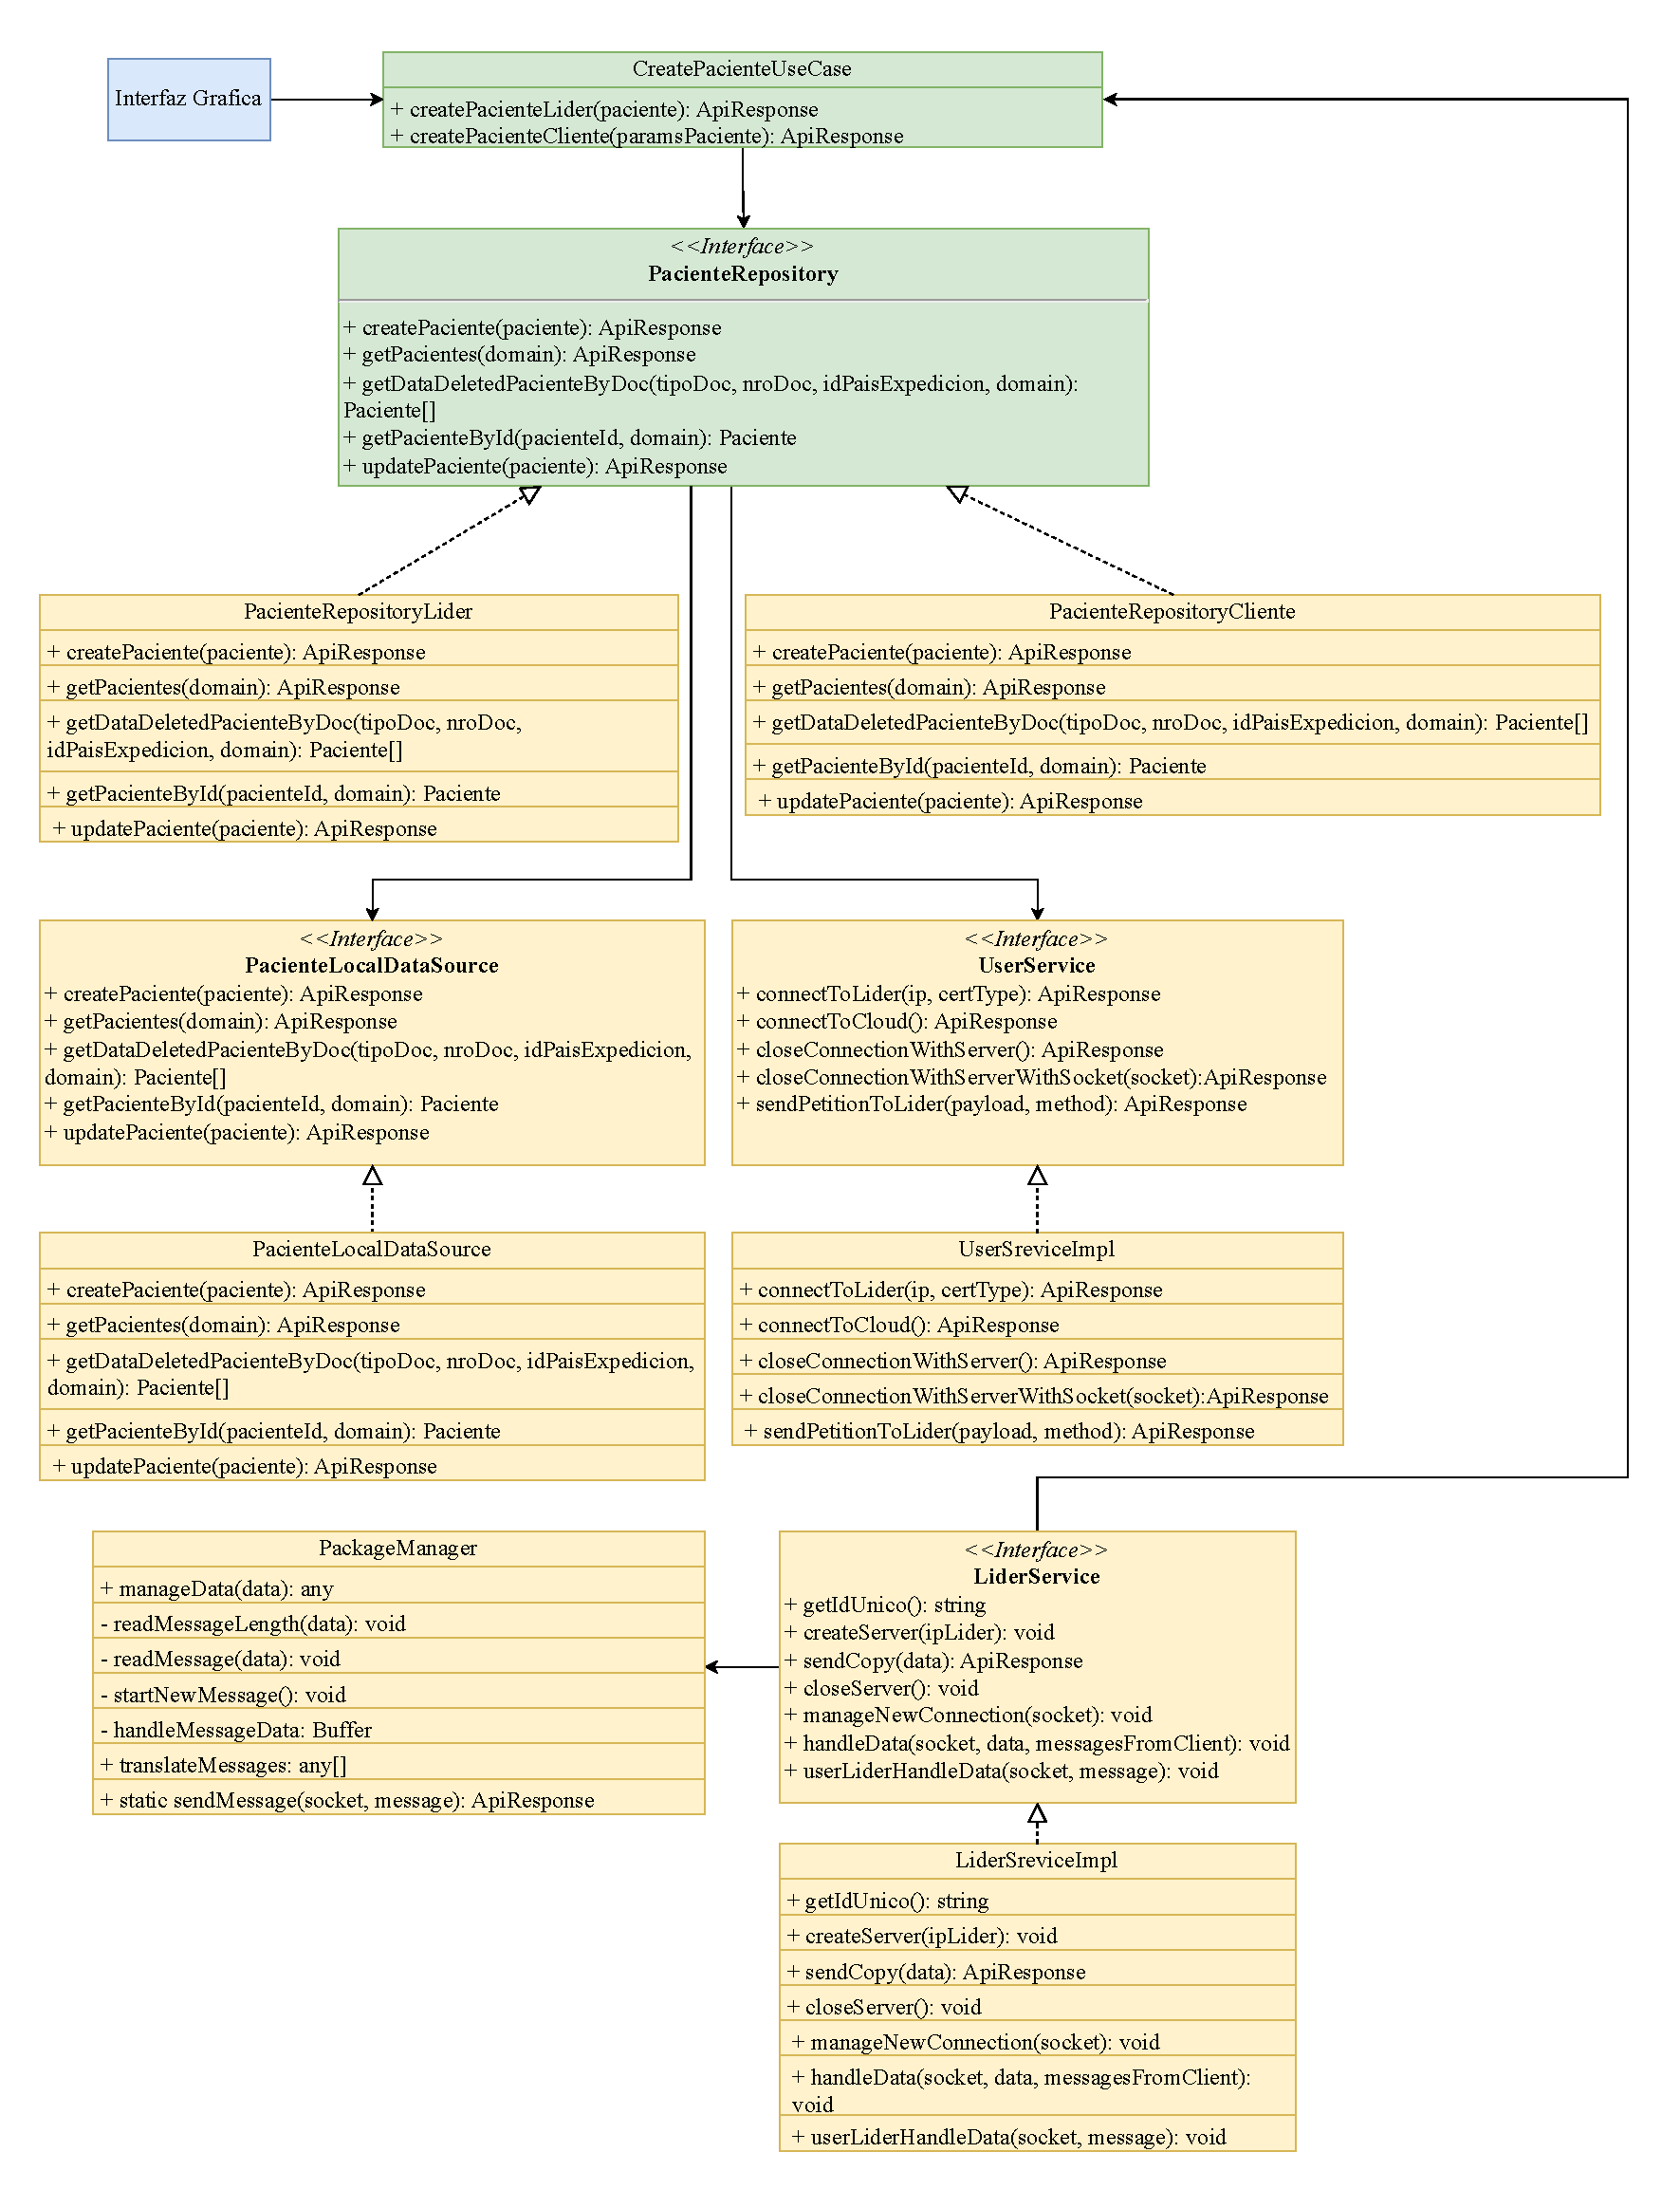
\includegraphics[width=\textwidth, height=\textheight, keepaspectratio]{Imagenes/Implementacion/DiagramaClasesAdmPaciente.pdf}
    \caption{Diagrama de clases del caso de uso \textit{Admisión Paciente}}
    \label{fig:diagClasesAdmPaciente}
\end{figure}

A continuación se procede a explicar el caso de uso \textit{Admisión paciente} con el diagrama de clases de la Figura \ref{fig:diagClasesAdmPaciente}, ademas es recomendable considerar la especificación del diagrama de actividades de la Figura \ref{fig:diagActAdmPaciente}:

\begin{enumerate}
    \item A través de la \textbf{interfaz gráfica}, el usuario utiliza el caso de uso con el método\\ \texttt{createPacienteCliente} de la clase \textbf{CreatePacienteUseCase}.
    
    \item El método \texttt{createPacienteCliente} realiza la actividad ``Generar petición'' y la envía a través de \textbf{UserServiceImpl} con el método \texttt{sendPetitionToLider}. Para el envío se hace uso del repositorio \textbf{PacienteRepositoryCliente} como intermediario entre el caso de uso y el servicio.

    \item El dispositivo de niebla recibe la petición en el método \texttt{handleData} de \textbf{LiderServiceImpl}, el cual contiene el socket del servidor a través del cual recibe los mensajes. Luego, interpreta el mensaje haciendo uso de \textbf{PackageManager} y ejecuta el caso de uso con el método\\ \texttt{createPacienteLider}, el cual se encarga de realizar la tarea ``Validar datos del dispositivo de borde''.

    \item El dispositivo de niebla, a través del repositorio \textbf{PacienteRepositoryLider}, utiliza el método \texttt{createPaciente} correspondiente a la implementación \textbf{PacienteLocalDataSource} el cual realiza las tareas de ``Generar Paciente'' y almacenarlo localmente.

    \item El dispositivo de niebla envía la respuesta al de borde haciendo uso del mismo \textit{socket} previamente establecido en la conexión inicial.

    \item El dispositivo de niebla realiza la tarea de replicación de datos hacia la nube y los dispositivos de niebla que estén conectados a él, incluido el que realizó la solicitud con el método \texttt{sendCopy} de \textbf{LiderService}.

    \item Al recibir la réplica, los dispositivos de borde ejecutan el procedimiento encargado del almacenamiento de réplicas.
    
\end{enumerate}





\section{Evaluación de funcionamiento}
En la Figura \ref{fig:screensTest} se muestran las interfaces gráficas usadas para verificar el funcionamiento durante el desarrollo. Estas están compuestas por botones que se encuentran distribuidos en tres pantallas, la de \textit{Inicio de sesión}, la de \textit{Menú principal} y la de \textit{Convertir a dispositivo de niebla}.

\begin{figure}[h]
    \centering
    \begin{minipage}{.3\textwidth}
        \centering
        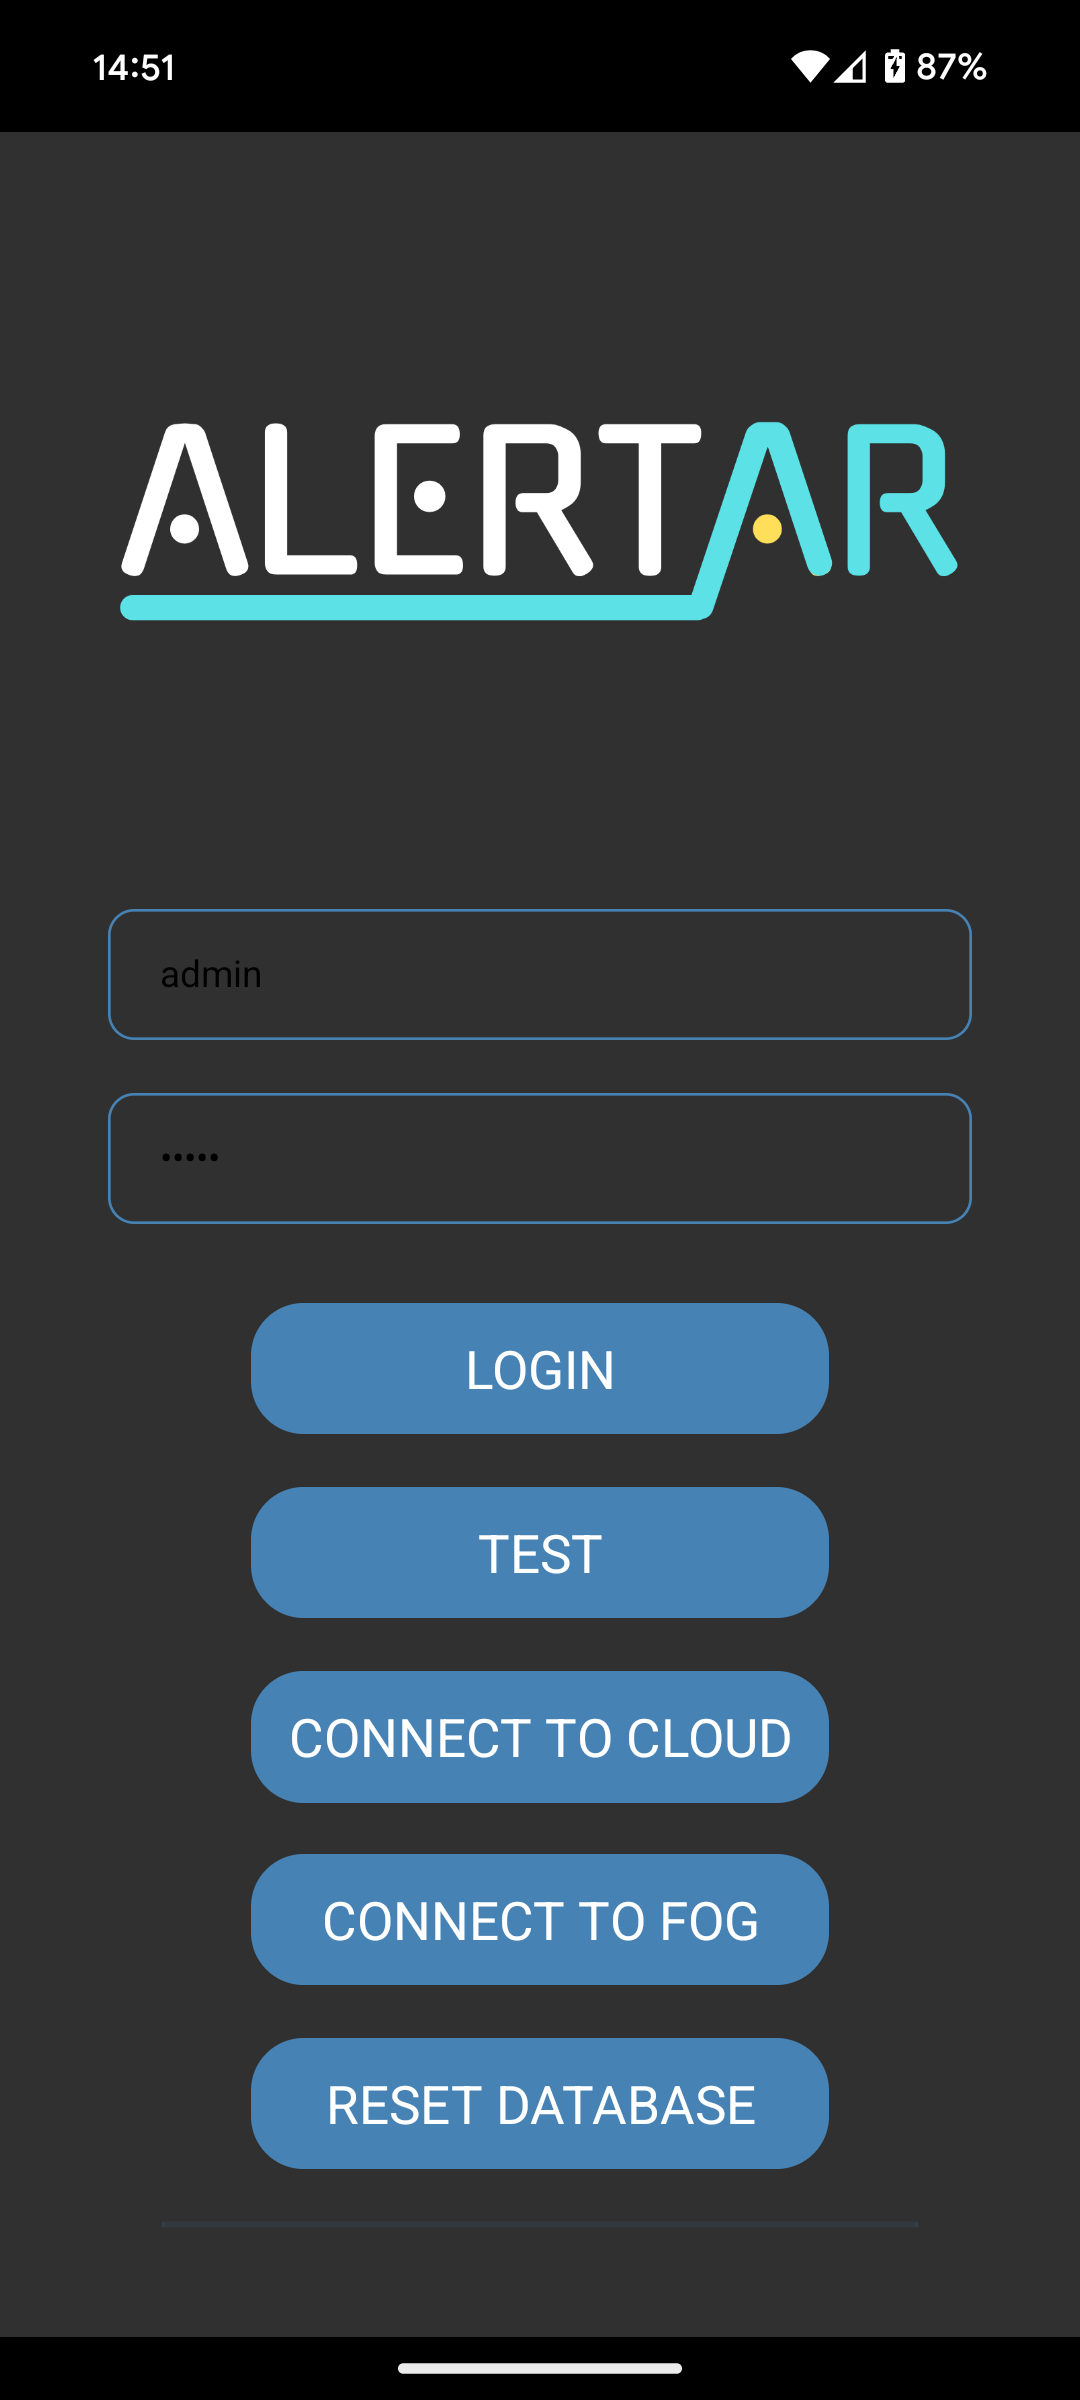
\includegraphics[width=\textwidth, keepaspectratio]{Imagenes/Implementacion/mainMenu.png}
 	
        \label{fig:screenLogin}
    \end{minipage}%
    \hfill
    \begin{minipage}{.3\textwidth}
        \centering
        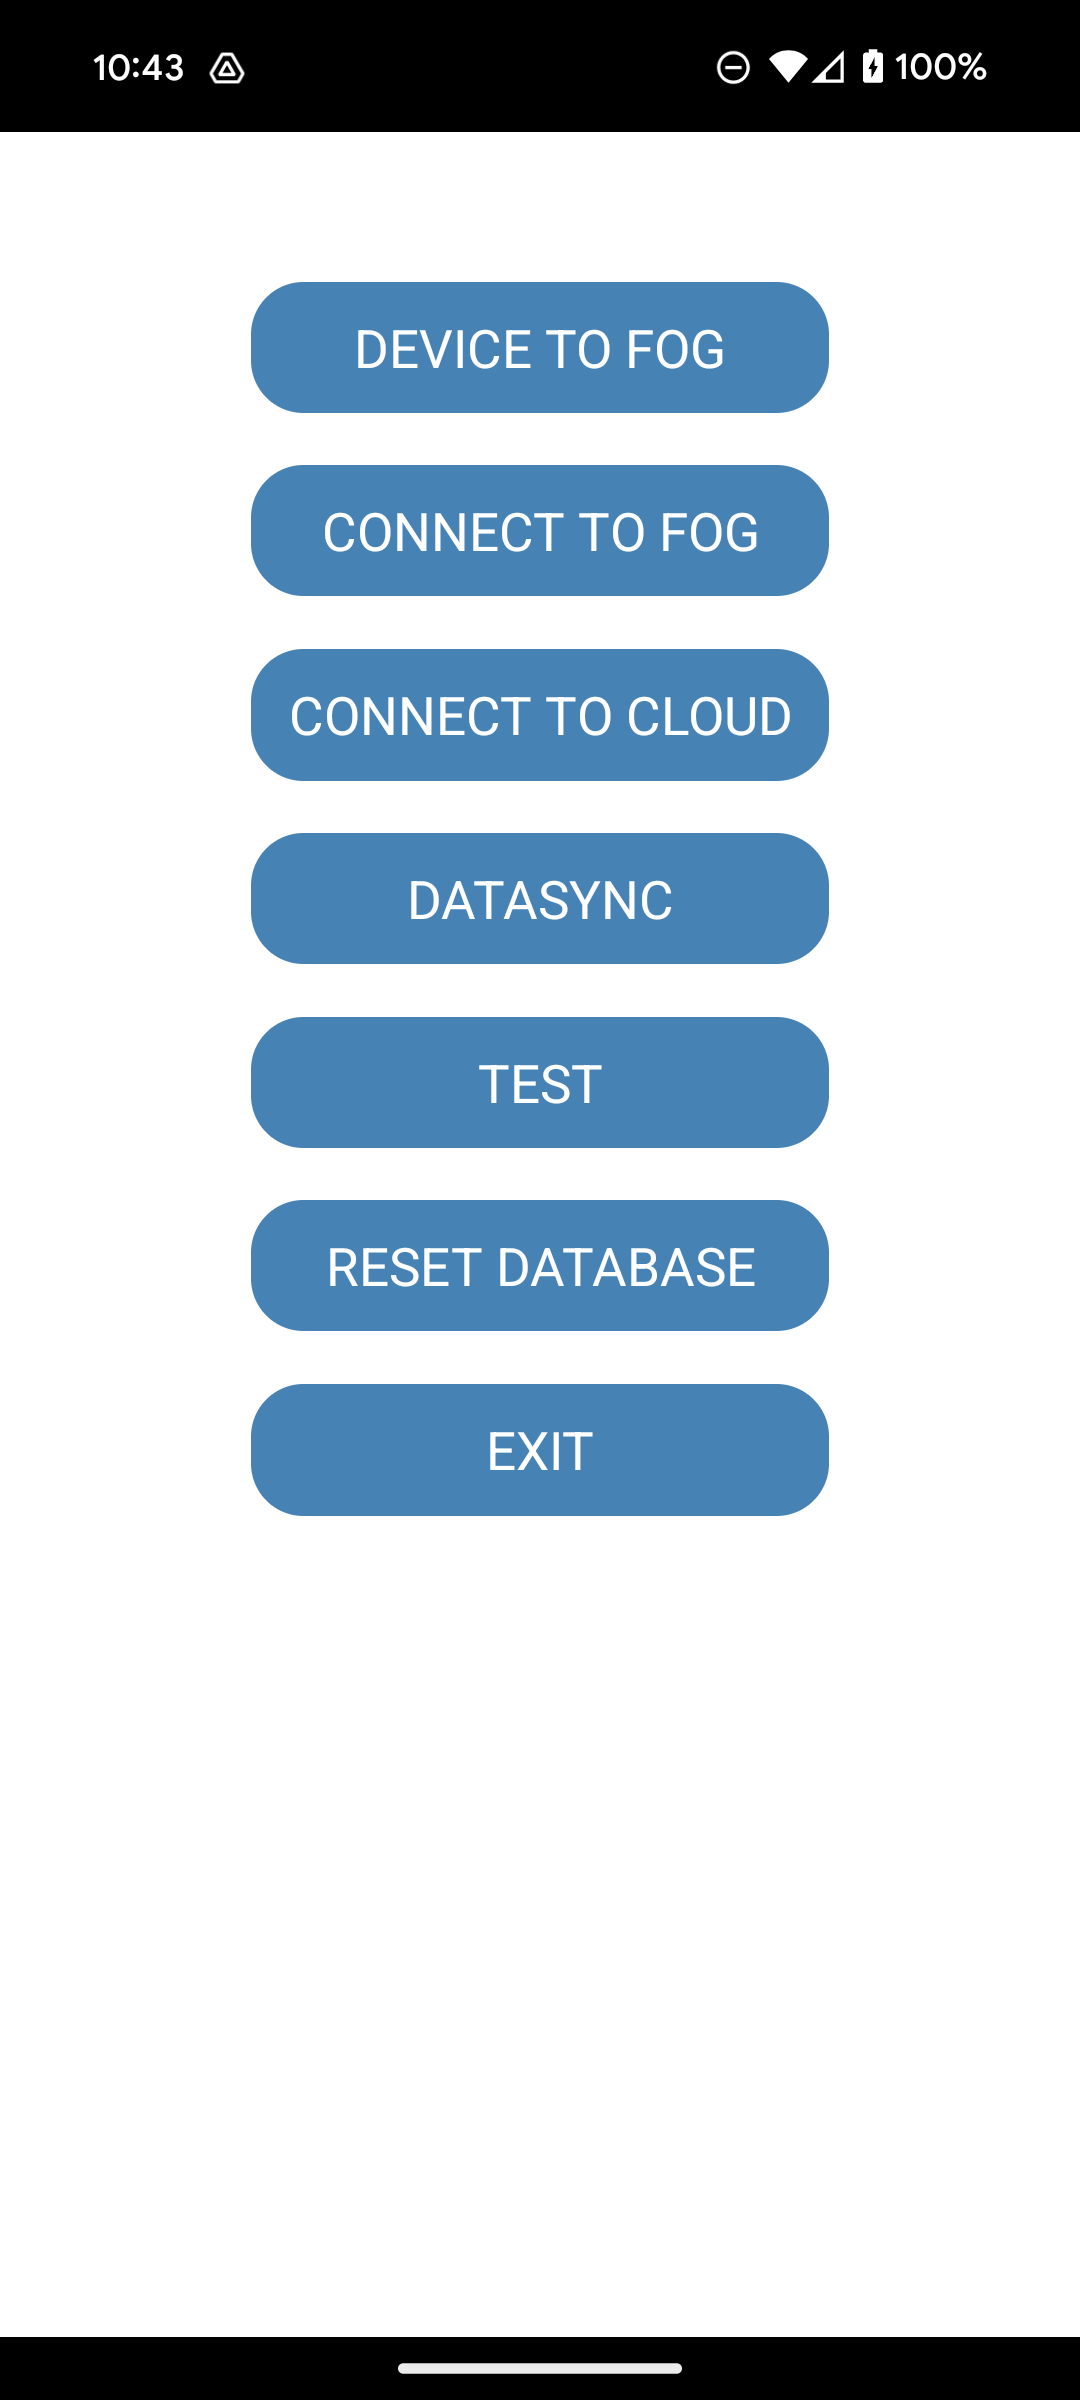
\includegraphics[width=\textwidth, keepaspectratio]{Imagenes/Implementacion/homeMenu.png}

        \label{fig:screenHome}
    \end{minipage}%
    \hfill
    \begin{minipage}{.3\textwidth}
        \centering
        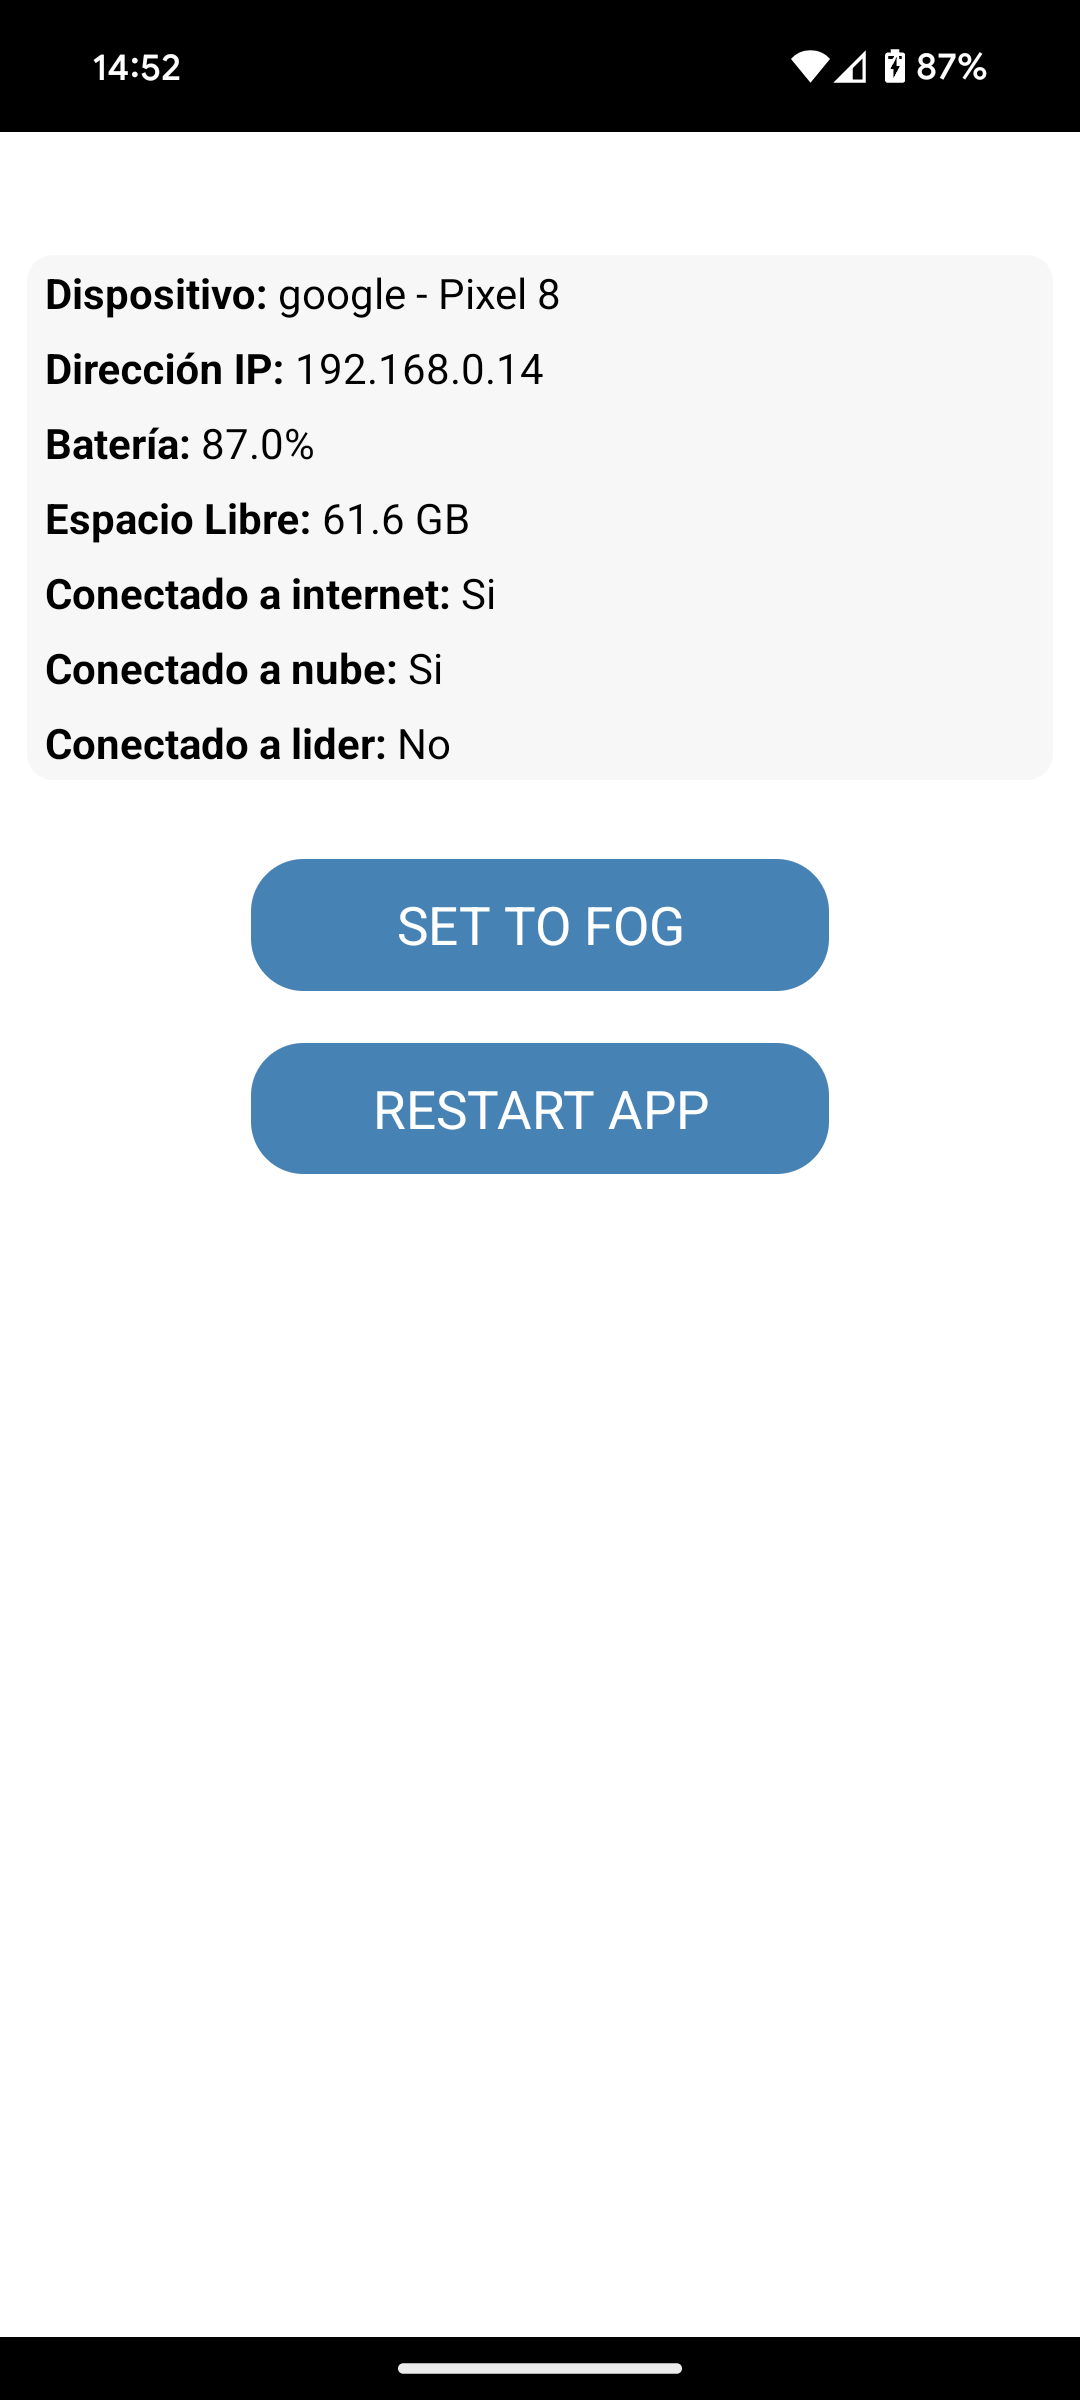
\includegraphics[width=\textwidth, keepaspectratio]{Imagenes/Implementacion/ConvertirALider.png}

        \label{fig:screenLider}
    \end{minipage}
    \caption{Pantallas \textit{Inicio de sesión}, \textit{Menú principal} y \textit{Convertir dispositivo a líder} utilizadas para la depuración en desarrollo}
    \label{fig:screensTest}
\end{figure}

Los botones al presionarse realizan acciones que derivan en llamados a casos de uso, los parámetros de estos llamados se especifican directamente en el código, evitando así la necesidad de interfaces gráficas con formularios para la carga de datos. Los botones realizan las siguientes acciones al presionarse:
\begin{itemize}
    \item \textbf{LOGIN: }ejecuta el caso de uso \textit{Iniciar sesión}.
    \item \textbf{TEST: }ejecuta un caso de uso especificado en el código para su evaluación.
    \item \textbf{CONNECT TO CLOUD: }realiza una conexión entre el dispositivo de borde con la nube.
    \item \textbf{CONNECT TO FOG: }realiza una conexión entre el dispositivo de borde con el dispositivo de niebla. Para esto, debe existir un dispositivo de niebla al cual conectarse, y el de borde ya debe tener el certificado e \textit{IP} del dispositivo de niebla para realizar la conexión.
    \item \textbf{RESET DATABASE: }restaura la base de datos a su estado original sin registros, excepto los registros correspondientes a los relojes lógicos de cada dominio que están inicializados en cero.
    \item \textbf{DEVICE TO FOG:} transición desde la pantalla \textit{Menú principal} a la pantalla  \textit{Convertir a dispositivo de niebla}.
    \item \textbf{SET TO FOG: }ejecuta el caso de uso \textit{Convertir a dispositivo de niebla}.
    \item \textbf{CLOSE CONNECTION: }desconecta al dispositivo de niebla, provocando que se corte la conexión de todos los dispositivos de borde y la nube con este.
    \item \textbf{DATASYNC: }el dispositivo de borde envía una solicitud para la sincronización de datos a la nube o al dispositivo de niebla al cual esté conectado.
    \item \textbf{EXIT: }transición desde la pantalla \textit{Menú principal} a la pantalla  \textit{Inicio de sesión}.
\end{itemize}


\subsection{Evaluación de la arquitectura}
Como se muestra en la Figura \ref{fig:arqGeneral} existen diferentes tipos de conexiones entre los componentes de la arquitectura. A causa de esto, se producen diferentes escenarios en cuanto al funcionamiento del sistema y estado de los datos. Los componentes del sistema pueden estar completamente operativos o algunos pueden fallar, en respuesta a esto el sistema debe mantenerse resiliente.

Los posibles escenarios se presentan en la Tabla \ref{tabla:evArq} y los resultados de la evaluación de cada uno fue positiva. En esta tabla, los dispositivos de borde se denominan "Borde", los dispositivos de niebla se mencionan como "Niebla", y los dispositivos que aún no tienen conexión se identifican simplemente como "Dispositivos".

En la primera columna se detalla, de manera resumida, el procedimiento que se está realizando a nivel núcleo de la aplicación. En la segunda columna se indica el tipo de conexión del dispositivo borde con el que se está operando, este puede estar conectado a la nube o a un dispositivo de niebla. En la tercera columna se contempla si existe conexión entre la nube y el dispositivo de niebla. En la cuarta columna se detalla el resultado esperado, que indica el estado de las bases de datos de los dispositivos participantes finalizado el procedimiento y, en caso de ser necesario, pasos intermedios que se deben cumplir antes de finalizar.


\begin{table}[h]

\captionof{table}{Evaluación del funcionamiento de la arquitectura}
\label{tabla:evArq} 
\begin{tabular}{|m{5cm}|m{2.5cm}|m{2cm}|m{5cm}|} \hline           
    \centering\textbf{Procedimiento} & \centering\textbf{Tipo conexión} & \centering\textbf{Hay conexión Nube $\Leftrightarrow$ Niebla} & \begin{center}
        \textbf{Resultado esperado}
    \end{center}  \\
    
    \hline Dispositivo se conecta a la nube, hace el \textit{dataSync}, se convierte en Niebla de un sector & Borde $\Leftrightarrow$ Nube & Sí & Se copia la BD de la nube en el nuevo dispositivo Niebla  \\ 
    %\hline El líder hace un \textit{insert} de un paciente & Cliente $\Leftrightarrow$ Nube & Sí & Se inserta un nuevo paciente en líder, nube y clientes & OK \\ 
    \hline El dispositivo de Borde hace un \textit{insert} de un paciente & Borde $\Leftrightarrow$ Nube & Sí & Se inserta un nuevo paciente en Niebla, Nube y Bordes\\
    \hline Borde hace un \textit{insert} de un paciente & Borde $\Leftrightarrow$ Nube & No & Mensaje de error ya que no hay acceso a la copia primaria de Niebla. \\
    \hline Dispositivo de borde se conecta a un dispositivo de Niebla, una vez es Borde hace \textit{dataSync} & Borde $\Leftrightarrow$ Niebla & Sí & Se copia la BD del Niebla en el dispositivo Borde \\
    %\hline Líder hace un \textit{insert} de un paciente & Cliente $\Leftrightarrow$ Líder & Sí & Se inserta un nuevo dato en líder, nube y clientes & OK \\
    \hline Borde hace un \textit{insert} de un paciente & Borde $\Leftrightarrow$ Niebla & Sí & Se inserta un nuevo paciente en Niebla, nube y Bordes \\
    \hline Borde hace un \textit{insert} de un paciente & Borde $\Leftrightarrow$ Niebla & No & Se inserta un nuevo paciente en Niebla y Bordes. Una vez que se restablece la conexión Nube $\Leftrightarrow$ Niebla, se sincroniza el dispositivo de niebla con la nube \\
    \hline\end{tabular} 

\end{table}

\subsection{Evaluación del mecanismo de detección de pérdida de conectividad}
    En la Figura \ref{fig:testConexion} se presentan los diferentes tipos de conexión y los posibles fallos en el sistema ALERTAR. Estos fallos pueden ocurrir en la nube, en las conexiones o en los dispositivos móviles que actúan como bordes o niebla. Los fallos en la nube o en los dispositivos móviles se consideran como una interrupción total de sus servicios, esto ocurre cuando se cierra la aplicación, cuando un dispositivo se queda sin batería o algún otro tipo de fallo no relacionado a la conectividad. Por otro lado, los fallos de conexión se deben a la pérdida de conectividad de cada dispositivo. Por ejemplo, si un dispositivo pierde señal o se queda sin datos, se considera una falla en su lado de la conexión.
    
    \begin{figure}
        \centering
        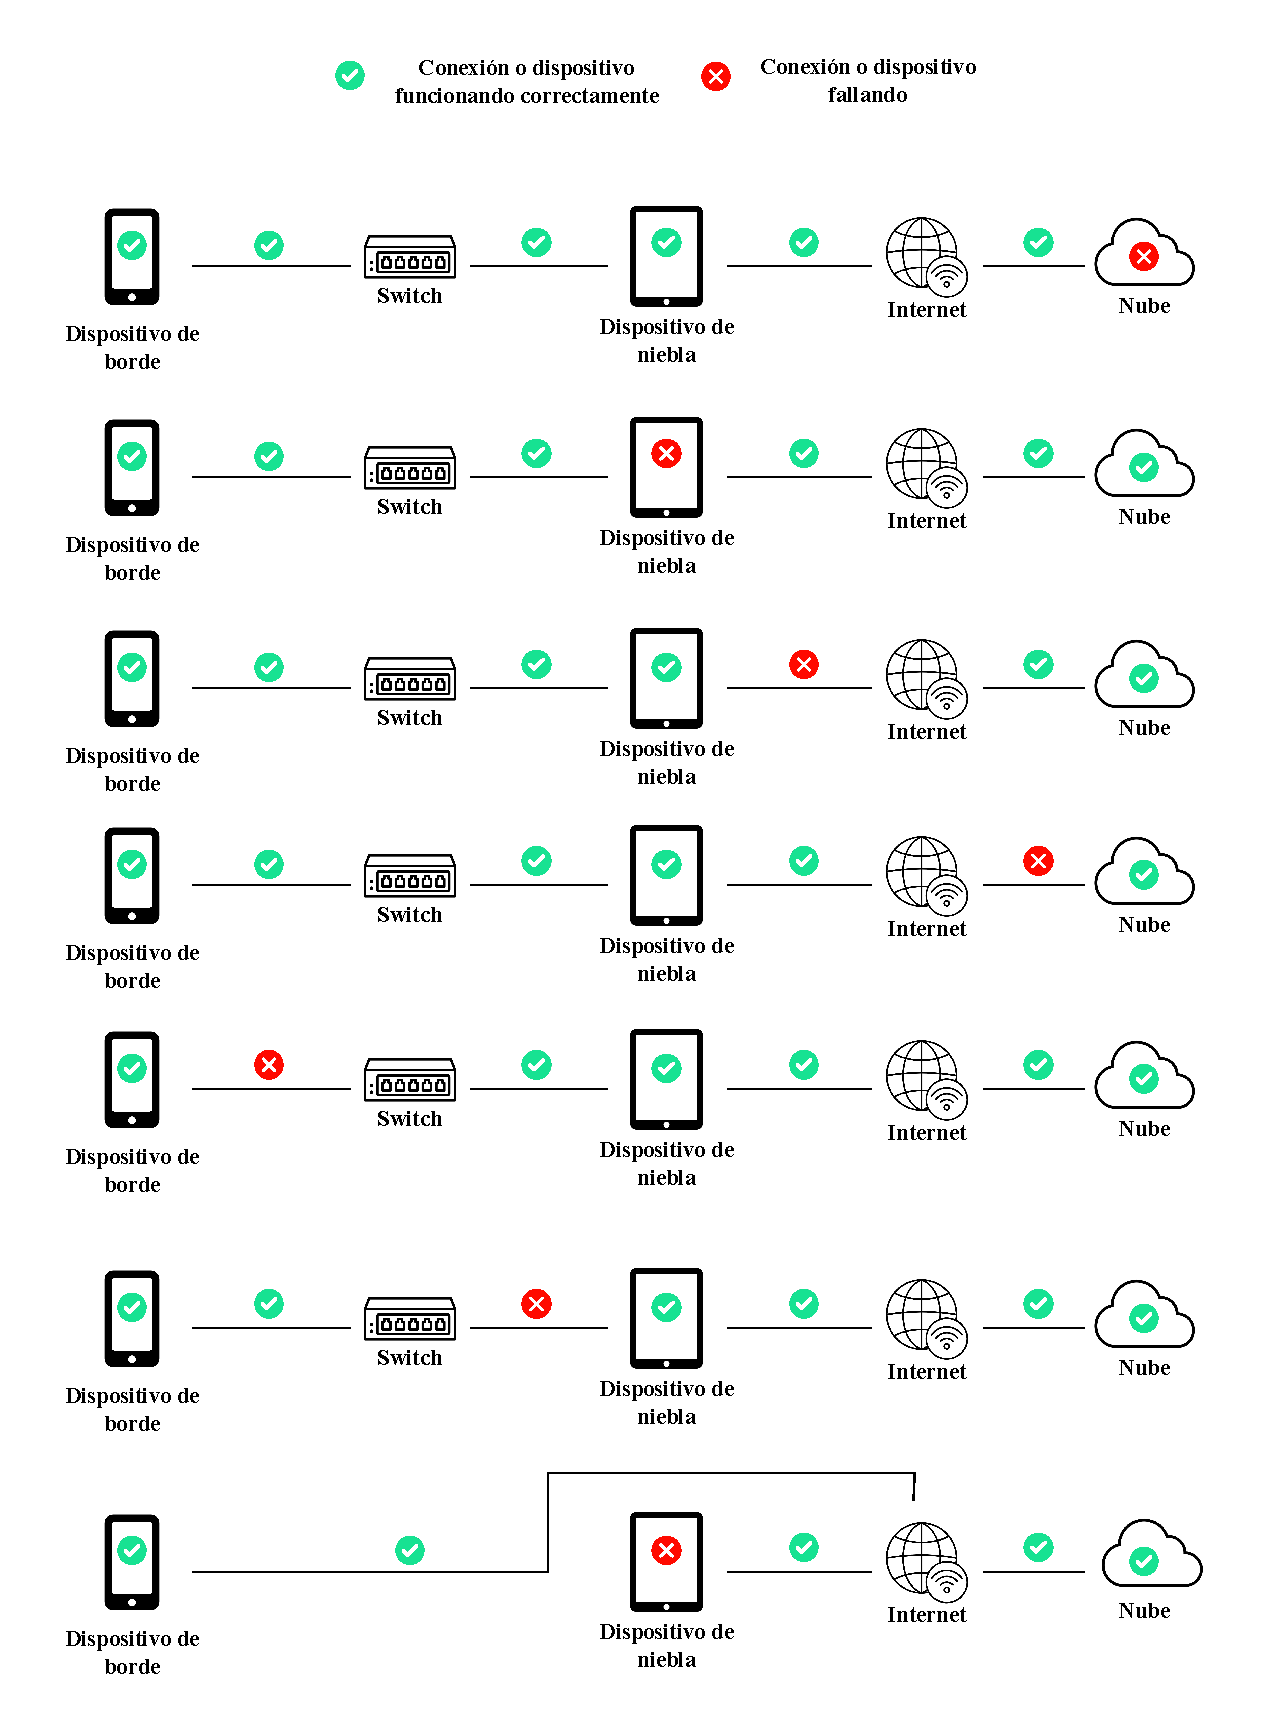
\includegraphics[width=\textwidth, height=\textheight, keepaspectratio]{Imagenes/Test/Conexiones.pdf}
        \caption{Tipos de conexión y sus posibles fallos en el sistema ALERTAR}
        \label{fig:testConexion}
    \end{figure}
    
    Se evaluaron todas las posibles combinaciones de fallos. Siempre se comenzó con el sistema totalmente operativo, luego se forzó uno por uno los diferentes tipos de fallos y se verificó que los dispositivos móviles fueran capaces de detectarlos. Posteriormente, se restableció el funcionamiento para comprobar que el sistema se recupera adecuadamente y volviera a estar operativo.
    
    A partir de esta evaluación se verificó que el mecanismo de detección de pérdida de conectividad y recuperación implementado en dispositivos móviles funciona correctamente, asegurando la recuperación del sistema ante fallos de dispositivos o conectividad.

\section{Mejoras al diseño arquitectónico}

El desarrollo de este prototipo básico permitió identificar diversas necesidades y aspectos a mejorar en el diseño arquitectónico. A través de la experiencia práctica de implementación, se detectaron ciertas limitaciones y oportunidades de mejora de diseño que pueden guiar futuras iteraciones del sistema.

\subsubsection{Separación de responsabilidades en la capa de datos}

Durante la implementación se observó que la capa de datos concentra responsabilidades heterogéneas que podrían beneficiarse de una mayor separación. Específicamente, la gestión de comunicaciones de red (como el manejo de sockets, conexiones TLS y protocolos de transporte) se encuentra mezclada con las responsabilidades relativas a una capa de datos, es decir acceso a bases de datos, repositorios y fuentes de datos. Esta mezcla dificulta el mantenimiento y la evolución independiente de estos aspectos.

Una mejora arquitectónica sería considerar la separación de las responsabilidades de comunicación de red en una capa específica, permitiendo que la capa de datos se enfoque exclusivamente en la gestión de datos y persistencia.

\subsubsection{Acoplamiento entre casos de uso y repositorios}

El diseño actual presenta múltiples repositorios específicos por separado. Esto implica la necesidad de especificar transacciones de base de datos sobre la implementación de estos repositorios. Estas transacciones son necesarias para ejecutar, de forma atómica, operaciones que involucren múltiples repositorios o fuentes de datos. De esta forma, el repositorio asume responsabilidades que trascienden su función primaria de orquestación de casos de uso, ya que se adentra en el manejo directo de detalles técnicos de persistencia. Esta mezcla de responsabilidades genera un acoplamiento fuerte entre la lógica de negocio y los mecanismos específicos de almacenamiento y acceso a datos ya que se violan los principios de responsabilidad única y separación de capas.

Dada la necesidad de manejar transacciones que involucren múltiples repositorios, se podría considerar la introducción de un gestor de repositorios. Este componente adicional se encargaría de coordinar las operaciones entre los diferentes repositorios mediante transacciones de negocio atómicas, permitiendo que cada uno mantenga su enfoque en la gestión de datos sin asumir responsabilidades técnicas relacionadas con la gestión de transacciones de bases de datos o detalles específicos de persistencia.

%todo DUDA: queda clara la diferencia entre transaccion de negocio y transacción de base de datos?
%\subsubsection{Gestión de roles de dispositivos en casos de uso}

%Durante el desarrollo se evidenció que los dispositivos de niebla y de borde presentan comportamientos distintos al ejecutar los mismos casos de uso. La implementación actual maneja estas diferencias dentro de cada caso implementando un método específico para cada tipo de dispositivo (niebla o borde), lo que genera complejidad a la hora de interpretar el código y flujo del sistema.

%Una aproximación alternativa sería considerar implementaciones específicas de casos de uso para cada tipo de dispositivo haciendo uso de una interfaz, permitiendo una lógica más clara y mantenible para cada contexto de ejecución.
